% Options for packages loaded elsewhere
\PassOptionsToPackage{unicode}{hyperref}
\PassOptionsToPackage{hyphens}{url}
%
\documentclass[
]{article}
\usepackage{amsmath,amssymb}
\usepackage{lmodern}
\usepackage{iftex}
\ifPDFTeX
  \usepackage[T1]{fontenc}
  \usepackage[utf8]{inputenc}
  \usepackage{textcomp} % provide euro and other symbols
\else % if luatex or xetex
  \usepackage{unicode-math}
  \defaultfontfeatures{Scale=MatchLowercase}
  \defaultfontfeatures[\rmfamily]{Ligatures=TeX,Scale=1}
\fi
% Use upquote if available, for straight quotes in verbatim environments
\IfFileExists{upquote.sty}{\usepackage{upquote}}{}
\IfFileExists{microtype.sty}{% use microtype if available
  \usepackage[]{microtype}
  \UseMicrotypeSet[protrusion]{basicmath} % disable protrusion for tt fonts
}{}
\makeatletter
\@ifundefined{KOMAClassName}{% if non-KOMA class
  \IfFileExists{parskip.sty}{%
    \usepackage{parskip}
  }{% else
    \setlength{\parindent}{0pt}
    \setlength{\parskip}{6pt plus 2pt minus 1pt}}
}{% if KOMA class
  \KOMAoptions{parskip=half}}
\makeatother
\usepackage{xcolor}
\usepackage[margin=1in]{geometry}
\usepackage{color}
\usepackage{fancyvrb}
\newcommand{\VerbBar}{|}
\newcommand{\VERB}{\Verb[commandchars=\\\{\}]}
\DefineVerbatimEnvironment{Highlighting}{Verbatim}{commandchars=\\\{\}}
% Add ',fontsize=\small' for more characters per line
\usepackage{framed}
\definecolor{shadecolor}{RGB}{248,248,248}
\newenvironment{Shaded}{\begin{snugshade}}{\end{snugshade}}
\newcommand{\AlertTok}[1]{\textcolor[rgb]{0.94,0.16,0.16}{#1}}
\newcommand{\AnnotationTok}[1]{\textcolor[rgb]{0.56,0.35,0.01}{\textbf{\textit{#1}}}}
\newcommand{\AttributeTok}[1]{\textcolor[rgb]{0.77,0.63,0.00}{#1}}
\newcommand{\BaseNTok}[1]{\textcolor[rgb]{0.00,0.00,0.81}{#1}}
\newcommand{\BuiltInTok}[1]{#1}
\newcommand{\CharTok}[1]{\textcolor[rgb]{0.31,0.60,0.02}{#1}}
\newcommand{\CommentTok}[1]{\textcolor[rgb]{0.56,0.35,0.01}{\textit{#1}}}
\newcommand{\CommentVarTok}[1]{\textcolor[rgb]{0.56,0.35,0.01}{\textbf{\textit{#1}}}}
\newcommand{\ConstantTok}[1]{\textcolor[rgb]{0.00,0.00,0.00}{#1}}
\newcommand{\ControlFlowTok}[1]{\textcolor[rgb]{0.13,0.29,0.53}{\textbf{#1}}}
\newcommand{\DataTypeTok}[1]{\textcolor[rgb]{0.13,0.29,0.53}{#1}}
\newcommand{\DecValTok}[1]{\textcolor[rgb]{0.00,0.00,0.81}{#1}}
\newcommand{\DocumentationTok}[1]{\textcolor[rgb]{0.56,0.35,0.01}{\textbf{\textit{#1}}}}
\newcommand{\ErrorTok}[1]{\textcolor[rgb]{0.64,0.00,0.00}{\textbf{#1}}}
\newcommand{\ExtensionTok}[1]{#1}
\newcommand{\FloatTok}[1]{\textcolor[rgb]{0.00,0.00,0.81}{#1}}
\newcommand{\FunctionTok}[1]{\textcolor[rgb]{0.00,0.00,0.00}{#1}}
\newcommand{\ImportTok}[1]{#1}
\newcommand{\InformationTok}[1]{\textcolor[rgb]{0.56,0.35,0.01}{\textbf{\textit{#1}}}}
\newcommand{\KeywordTok}[1]{\textcolor[rgb]{0.13,0.29,0.53}{\textbf{#1}}}
\newcommand{\NormalTok}[1]{#1}
\newcommand{\OperatorTok}[1]{\textcolor[rgb]{0.81,0.36,0.00}{\textbf{#1}}}
\newcommand{\OtherTok}[1]{\textcolor[rgb]{0.56,0.35,0.01}{#1}}
\newcommand{\PreprocessorTok}[1]{\textcolor[rgb]{0.56,0.35,0.01}{\textit{#1}}}
\newcommand{\RegionMarkerTok}[1]{#1}
\newcommand{\SpecialCharTok}[1]{\textcolor[rgb]{0.00,0.00,0.00}{#1}}
\newcommand{\SpecialStringTok}[1]{\textcolor[rgb]{0.31,0.60,0.02}{#1}}
\newcommand{\StringTok}[1]{\textcolor[rgb]{0.31,0.60,0.02}{#1}}
\newcommand{\VariableTok}[1]{\textcolor[rgb]{0.00,0.00,0.00}{#1}}
\newcommand{\VerbatimStringTok}[1]{\textcolor[rgb]{0.31,0.60,0.02}{#1}}
\newcommand{\WarningTok}[1]{\textcolor[rgb]{0.56,0.35,0.01}{\textbf{\textit{#1}}}}
\usepackage{graphicx}
\makeatletter
\def\maxwidth{\ifdim\Gin@nat@width>\linewidth\linewidth\else\Gin@nat@width\fi}
\def\maxheight{\ifdim\Gin@nat@height>\textheight\textheight\else\Gin@nat@height\fi}
\makeatother
% Scale images if necessary, so that they will not overflow the page
% margins by default, and it is still possible to overwrite the defaults
% using explicit options in \includegraphics[width, height, ...]{}
\setkeys{Gin}{width=\maxwidth,height=\maxheight,keepaspectratio}
% Set default figure placement to htbp
\makeatletter
\def\fps@figure{htbp}
\makeatother
\setlength{\emergencystretch}{3em} % prevent overfull lines
\providecommand{\tightlist}{%
  \setlength{\itemsep}{0pt}\setlength{\parskip}{0pt}}
\setcounter{secnumdepth}{-\maxdimen} % remove section numbering
\ifLuaTeX
  \usepackage{selnolig}  % disable illegal ligatures
\fi
\IfFileExists{bookmark.sty}{\usepackage{bookmark}}{\usepackage{hyperref}}
\IfFileExists{xurl.sty}{\usepackage{xurl}}{} % add URL line breaks if available
\urlstyle{same} % disable monospaced font for URLs
\hypersetup{
  pdftitle={Assignment 1 - Language development in autistic and neurotypical children},
  hidelinks,
  pdfcreator={LaTeX via pandoc}}

\title{Assignment 1 - Language development in autistic and neurotypical
children}
\author{}
\date{\vspace{-2.5em}}

\begin{document}
\maketitle

\hypertarget{assignment-1---language-development-in-autistic-and-neurotypical-children}{%
\section{Assignment 1 - Language development in autistic and
neurotypical
children}\label{assignment-1---language-development-in-autistic-and-neurotypical-children}}

\hypertarget{quick-recap}{%
\subsection{Quick recap}\label{quick-recap}}

Autism Spectrum Disorder is often related to language impairment.
However, this phenomenon has rarely been empirically traced in detail:
i) relying on actual naturalistic language production, ii) over extended
periods of time.

We therefore videotaped circa 30 kids with ASD and circa 30 comparison
kids (matched by linguistic performance at visit 1) for ca. 30 minutes
of naturalistic interactions with a parent. We repeated the data
collection 6 times per kid, with 4 months between each visit. We
transcribed the data and counted: i) the amount of words that each kid
uses in each video. Same for the parent. ii) the amount of unique words
that each kid uses in each video. Same for the parent. iii) the amount
of morphemes per utterance (Mean Length of Utterance) displayed by each
child in each video. Same for the parent.

This data is in the file you prepared in the previous class, but you can
also find it
here:\url{https://www.dropbox.com/s/d6eerv6cl6eksf3/data_clean.csv?dl=0}

\hypertarget{the-structure-of-the-assignment}{%
\subsection{The structure of the
assignment}\label{the-structure-of-the-assignment}}

We will be spending a few weeks with this assignment. In particular, we
will:

Part 1) simulate data in order to better understand the model we need to
build, and to better understand how much data we would have to collect
to run a meaningful study (precision analysis)

Part 2) analyze our empirical data and interpret the inferential results

Part 3) use your model to predict the linguistic trajectory of new
children and assess the performance of the model based on that.

As you work through these parts, you will have to produce a written
document (separated from the code) answering the following questions:

Q1 - Briefly describe your simulation process, its goals, and what you
have learned from the simulation. Add at least a plot showcasing the
results of the simulation. Make a special note on sample size
considerations: how much data do you think you will need? what else
could you do to increase the precision of your estimates?

Q2 - Briefly describe the empirical data and how they compare to what
you learned from the simulation (what can you learn from them?). Briefly
describe your model(s) and model quality. Report the findings: how does
development differ between autistic and neurotypical children (N.B.
remember to report both population and individual level findings)? which
additional factors should be included in the model? Add at least one
plot showcasing your findings.

Q3 - Given the model(s) from Q2, how well do they predict the data?
Discuss both in terms of absolute error in training vs testing; and in
terms of characterizing the new kids' language development as typical or
in need of support.

Below you can find more detailed instructions for each part of the
assignment.

\hypertarget{part-1---simulating-data}{%
\subsection{Part 1 - Simulating data}\label{part-1---simulating-data}}

Before we even think of analyzing the data, we should make sure we
understand the problem, and we plan the analysis. To do so, we need to
simulate data and analyze the simulated data (where we know the ground
truth).

In particular, let's imagine we have n autistic and n neurotypical
children. We are simulating their average utterance length (Mean Length
of Utterance or MLU) in terms of words, starting at Visit 1 and all the
way to Visit 6. In other words, we need to define a few parameters: -
average MLU for ASD (population mean) at Visit 1 and average individual
deviation from that (population standard deviation) - average MLU for TD
(population mean) at Visit 1 and average individual deviation from that
(population standard deviation) - average change in MLU by visit for ASD
(population mean) and average individual deviation from that (population
standard deviation) - average change in MLU by visit for TD (population
mean) and average individual deviation from that (population standard
deviation) - an error term. Errors could be due to measurement,
sampling, all sorts of noise.

Note that this makes a few assumptions: population means are exact
values; change by visit is linear (the same between visit 1 and 2 as
between visit 5 and 6). This is fine for the exercise. In real life
research, you might want to vary the parameter values much more, relax
those assumptions and assess how these things impact your inference.

We go through the literature and we settle for some values for these
parameters: - average MLU for ASD and TD: 1.5 (remember the populations
are matched for linguistic ability at first visit) - average individual
variability in initial MLU for ASD 0.5; for TD 0.3 (remember ASD tends
to be more heterogeneous) - average change in MLU for ASD: 0.4; for TD
0.6 (ASD is supposed to develop less) - average individual variability
in change for ASD 0.4; for TD 0.2 (remember ASD tends to be more
heterogeneous) - error is identified as 0.2

This would mean that on average the difference between ASD and TD
participants is 0 at visit 1, 0.2 at visit 2, 0.4 at visit 3, 0.6 at
visit 4, 0.8 at visit 5 and 1 at visit 6.

With these values in mind, simulate data, plot the data (to check
everything is alright); and set up an analysis pipeline.

Remember the usual bayesian workflow: - define the formula - define the
prior - prior predictive checks - fit the model - model quality checks:
traceplots, divergences, rhat, effective samples - model quality checks:
posterior predictive checks, prior-posterior update checks - model
comparison

Once the pipeline is in place, loop through different sample sizes to
assess how much data you would need to collect. N.B. for inspiration on
how to set this up, check the tutorials by Kurz that are linked in the
syllabus.

BONUS questions for Part 1: what if the difference between ASD and TD
was 0? how big of a sample size would you need? What about different
effect sizes, and different error terms?

Bryan \#\#\# Simulating data To make beta values between each visit we
would need the standard diviation between visits

\begin{Shaded}
\begin{Highlighting}[]
\NormalTok{average\_mlu }\OtherTok{\textless{}{-}} \FunctionTok{log}\NormalTok{(}\FloatTok{1.5}\NormalTok{)}
\NormalTok{ sd\_mlu\_asd }\OtherTok{\textless{}{-}} \FunctionTok{log}\NormalTok{(}\FloatTok{1.5+0.5}\NormalTok{)}\SpecialCharTok{{-}}\FunctionTok{log}\NormalTok{(}\FloatTok{1.5}\NormalTok{)}
\NormalTok{ sd\_mlu\_td }\OtherTok{\textless{}{-}} \FunctionTok{log}\NormalTok{(}\FloatTok{1.5+0.3}\NormalTok{)}\SpecialCharTok{{-}}\FunctionTok{log}\NormalTok{(}\FloatTok{1.5}\NormalTok{)}
 
\NormalTok{ change\_mlu\_asd }\OtherTok{\textless{}{-}} \FloatTok{0.4}\SpecialCharTok{/}\FloatTok{1.5}
\NormalTok{ change\_mlu\_td }\OtherTok{\textless{}{-}} \FloatTok{0.6}\SpecialCharTok{/}\FloatTok{1.5}
\NormalTok{ change\_sd\_mlu\_asd }\OtherTok{\textless{}{-}} \FloatTok{0.4}\SpecialCharTok{*}\NormalTok{(}\FloatTok{0.4}\SpecialCharTok{/}\FloatTok{1.5}\NormalTok{)}
\NormalTok{ change\_sd\_mlu\_td }\OtherTok{\textless{}{-}} \FloatTok{0.2}\SpecialCharTok{*}\NormalTok{(}\FloatTok{0.6}\SpecialCharTok{/}\FloatTok{1.5}\NormalTok{)}
\NormalTok{ e }\OtherTok{\textless{}{-}} \FloatTok{0.2}

\NormalTok{n }\OtherTok{\textless{}{-}} \DecValTok{100}
\end{Highlighting}
\end{Shaded}

\begin{Shaded}
\begin{Highlighting}[]
\NormalTok{int\_asd }\OtherTok{\textless{}{-}} \FunctionTok{rnorm}\NormalTok{(n, }\AttributeTok{mean=}\NormalTok{average\_mlu, }\AttributeTok{sd=}\NormalTok{sd\_mlu\_asd)}
\NormalTok{int\_td }\OtherTok{\textless{}{-}} \FunctionTok{rnorm}\NormalTok{(n, }\AttributeTok{mean=}\NormalTok{average\_mlu, }\AttributeTok{sd=}\NormalTok{sd\_mlu\_td)}

\NormalTok{slope\_asd }\OtherTok{\textless{}{-}} \FunctionTok{rnorm}\NormalTok{(n, }\AttributeTok{mean=}\NormalTok{change\_mlu\_asd, }\AttributeTok{sd=}\NormalTok{change\_sd\_mlu\_asd)}
\NormalTok{slope\_td }\OtherTok{\textless{}{-}} \FunctionTok{rnorm}\NormalTok{(n, }\AttributeTok{mean =}\NormalTok{ change\_mlu\_td, }\AttributeTok{sd=}\NormalTok{change\_sd\_mlu\_td)}
\end{Highlighting}
\end{Shaded}

\begin{Shaded}
\begin{Highlighting}[]
\NormalTok{ sim\_data }\OtherTok{\textless{}{-}} 
   \FunctionTok{tibble}\NormalTok{(}\AttributeTok{diagnosis=}\FunctionTok{rep}\NormalTok{(}\FunctionTok{c}\NormalTok{(}\StringTok{\textquotesingle{}TD\textquotesingle{}}\NormalTok{, }\StringTok{\textquotesingle{}ASD\textquotesingle{}}\NormalTok{), }\AttributeTok{each=}\NormalTok{n)) }\SpecialCharTok{\%\textgreater{}\%} 
   \FunctionTok{mutate}\NormalTok{(}\AttributeTok{intercept=}\FunctionTok{ifelse}\NormalTok{(diagnosis}\SpecialCharTok{==}\StringTok{\textquotesingle{}TD\textquotesingle{}}\NormalTok{, int\_td, int\_asd)) }\SpecialCharTok{\%\textgreater{}\%} 
   \FunctionTok{mutate}\NormalTok{(}\AttributeTok{slope=}\FunctionTok{ifelse}\NormalTok{(diagnosis}\SpecialCharTok{==}\StringTok{\textquotesingle{}TD\textquotesingle{}}\NormalTok{, slope\_td, slope\_asd)) }\SpecialCharTok{\%\textgreater{}\%} 
   \FunctionTok{mutate}\NormalTok{(}\AttributeTok{error=}\FunctionTok{ifelse}\NormalTok{(diagnosis}\SpecialCharTok{==}\StringTok{\textquotesingle{}TD\textquotesingle{}}\NormalTok{, e, e)) }\SpecialCharTok{\%\textgreater{}\%} 
\NormalTok{   dplyr}\SpecialCharTok{::}\FunctionTok{mutate}\NormalTok{(}\AttributeTok{ID=}\FunctionTok{row\_number}\NormalTok{()) }\SpecialCharTok{\%\textgreater{}\%} 
   \FunctionTok{slice}\NormalTok{(}\FunctionTok{rep}\NormalTok{(}\DecValTok{1}\SpecialCharTok{:}\FunctionTok{n}\NormalTok{(), }\AttributeTok{each=}\DecValTok{6}\NormalTok{)) }\SpecialCharTok{\%\textgreater{}\%} 
   \FunctionTok{add\_column}\NormalTok{(}\AttributeTok{visit=}\FunctionTok{rep}\NormalTok{(}\FunctionTok{c}\NormalTok{(}\DecValTok{1}\NormalTok{,}\DecValTok{2}\NormalTok{,}\DecValTok{3}\NormalTok{,}\DecValTok{4}\NormalTok{,}\DecValTok{5}\NormalTok{,}\DecValTok{6}\NormalTok{), }\AttributeTok{times=}\NormalTok{n}\SpecialCharTok{+}\NormalTok{n))}
 
 \ControlFlowTok{for}\NormalTok{(i }\ControlFlowTok{in} \FunctionTok{seq}\NormalTok{(}\FunctionTok{nrow}\NormalTok{(sim\_data)))\{}
\NormalTok{   sim\_data}\SpecialCharTok{$}\NormalTok{MLU[i] }\OtherTok{\textless{}{-}} \FunctionTok{exp}\NormalTok{(}\FunctionTok{rnorm}\NormalTok{(}\DecValTok{1}\NormalTok{, sim\_data}\SpecialCharTok{$}\NormalTok{intercept[i]}\SpecialCharTok{+}\NormalTok{(sim\_data}\SpecialCharTok{$}\NormalTok{slope[i]}\SpecialCharTok{*}\NormalTok{(sim\_data}\SpecialCharTok{$}\NormalTok{visit[i]}\SpecialCharTok{{-}}\DecValTok{1}\NormalTok{)), sim\_data}\SpecialCharTok{$}\NormalTok{error[i]))}
\NormalTok{ \}}
\end{Highlighting}
\end{Shaded}

\begin{verbatim}
## Warning: Unknown or uninitialised column: `MLU`.
\end{verbatim}

\hypertarget{plot-simulated-data}{%
\subsubsection{plot simulated data}\label{plot-simulated-data}}

\begin{Shaded}
\begin{Highlighting}[]
\FunctionTok{ggplot}\NormalTok{(sim\_data, }\FunctionTok{aes}\NormalTok{(visit,MLU, }\AttributeTok{color=}\NormalTok{diagnosis, }\AttributeTok{group=}\NormalTok{ID))}\SpecialCharTok{+}
  \FunctionTok{theme\_bw}\NormalTok{()}\SpecialCharTok{+}
  \FunctionTok{geom\_point}\NormalTok{()}\SpecialCharTok{+}
  \FunctionTok{geom\_line}\NormalTok{(}\AttributeTok{alpha=}\FloatTok{0.3}\NormalTok{)}
\end{Highlighting}
\end{Shaded}

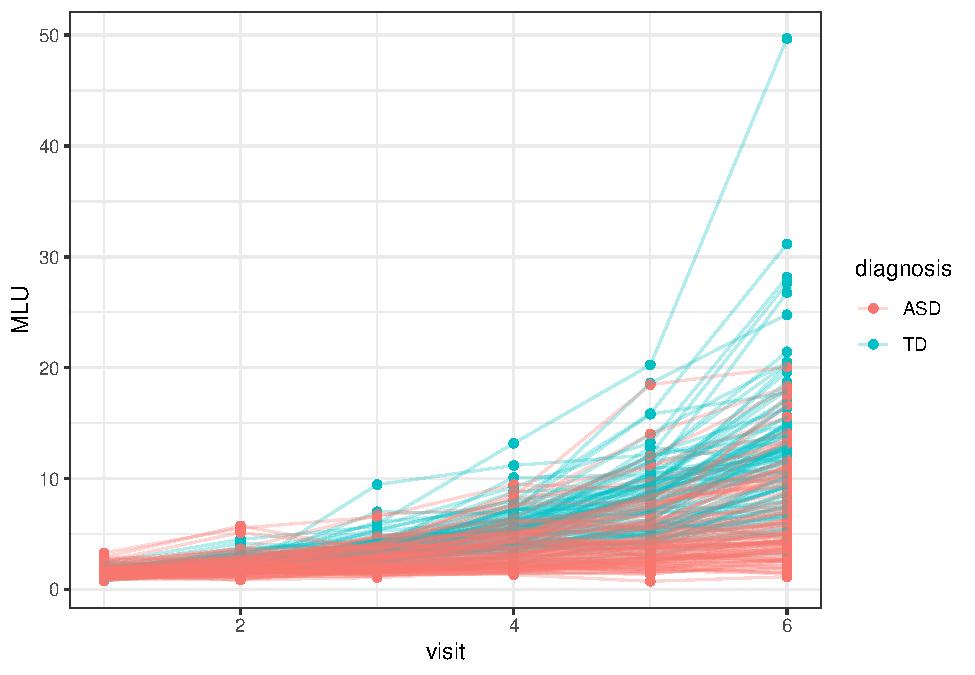
\includegraphics{assignment_1_final_files/figure-latex/unnamed-chunk-4-1.pdf}
\#\#Analysing simulated data

\#\#\#define formula

\begin{Shaded}
\begin{Highlighting}[]
\NormalTok{MLU\_f1 }\OtherTok{\textless{}{-}} \FunctionTok{bf}\NormalTok{(MLU }\SpecialCharTok{\textasciitilde{}} \DecValTok{0} \SpecialCharTok{+}\NormalTok{ diagnosis }\SpecialCharTok{+}\NormalTok{ diagnosis}\SpecialCharTok{:}\NormalTok{visit }\SpecialCharTok{+}\NormalTok{ (}\DecValTok{1} \SpecialCharTok{+}\NormalTok{ visit}\SpecialCharTok{|}\NormalTok{ID))}
\end{Highlighting}
\end{Shaded}

\begin{Shaded}
\begin{Highlighting}[]
\NormalTok{lognorm\_fam }\OtherTok{\textless{}{-}} \FunctionTok{brmsfamily}\NormalTok{(}\StringTok{\textquotesingle{}lognormal\textquotesingle{}}\NormalTok{, }\AttributeTok{bhaz =} \FunctionTok{list}\NormalTok{(}\AttributeTok{Boundary.knots=}\FunctionTok{c}\NormalTok{(}\SpecialCharTok{{-}}\DecValTok{1}\NormalTok{,}\DecValTok{31}\NormalTok{)))}
\end{Highlighting}
\end{Shaded}

\#\#\#Investigate and set priors

\begin{Shaded}
\begin{Highlighting}[]
\FunctionTok{get\_prior}\NormalTok{(}\AttributeTok{data =}\NormalTok{ sim\_data, }\AttributeTok{family =}\NormalTok{ lognorm\_fam, MLU\_f1)}
\end{Highlighting}
\end{Shaded}

\begin{verbatim}
##                 prior class               coef group resp dpar nlpar lb ub
##                (flat)     b                                               
##                (flat)     b       diagnosisASD                            
##                (flat)     b diagnosisASD:visit                            
##                (flat)     b        diagnosisTD                            
##                (flat)     b  diagnosisTD:visit                            
##                lkj(1)   cor                                               
##                lkj(1)   cor                       ID                      
##  student_t(3, 0, 2.5)    sd                                           0   
##  student_t(3, 0, 2.5)    sd                       ID                  0   
##  student_t(3, 0, 2.5)    sd          Intercept    ID                  0   
##  student_t(3, 0, 2.5)    sd              visit    ID                  0   
##  student_t(3, 0, 2.5) sigma                                           0   
##        source
##       default
##  (vectorized)
##  (vectorized)
##  (vectorized)
##  (vectorized)
##       default
##  (vectorized)
##       default
##  (vectorized)
##  (vectorized)
##  (vectorized)
##       default
\end{verbatim}

\begin{Shaded}
\begin{Highlighting}[]
\NormalTok{priors }\OtherTok{\textless{}{-}} \FunctionTok{c}\NormalTok{(}
\FunctionTok{prior}\NormalTok{(}\FunctionTok{normal}\NormalTok{(}\FloatTok{1.5}\NormalTok{,}\FloatTok{0.5}\NormalTok{),}\AttributeTok{class=}\NormalTok{b,}\AttributeTok{coef=}\StringTok{"diagnosisASD"}\NormalTok{),}
\FunctionTok{prior}\NormalTok{(}\FunctionTok{normal}\NormalTok{(}\FloatTok{1.5}\NormalTok{,}\FloatTok{0.3}\NormalTok{),}\AttributeTok{class=}\NormalTok{b,}\AttributeTok{coef=}\StringTok{"diagnosisTD"}\NormalTok{),}
\FunctionTok{prior}\NormalTok{(}\FunctionTok{normal}\NormalTok{(}\DecValTok{0}\NormalTok{,}\FloatTok{0.5}\NormalTok{),}\AttributeTok{class=}\NormalTok{b),}
\FunctionTok{prior}\NormalTok{(}\FunctionTok{normal}\NormalTok{(}\DecValTok{0}\NormalTok{,}\FloatTok{0.5}\NormalTok{),}\AttributeTok{class=}\NormalTok{sd),}
\FunctionTok{prior}\NormalTok{(}\FunctionTok{lkj}\NormalTok{(}\DecValTok{2}\NormalTok{),}\AttributeTok{class=}\NormalTok{cor))}
\end{Highlighting}
\end{Shaded}

\#\#\#Model using priors

\begin{Shaded}
\begin{Highlighting}[]
\NormalTok{MLU\_prior\_m1 }\OtherTok{\textless{}{-}} \FunctionTok{brm}\NormalTok{(}
\NormalTok{  MLU\_f1, }
  \AttributeTok{data =}\NormalTok{ sim\_data, }
  \AttributeTok{prior =}\NormalTok{ priors,}
  \AttributeTok{family =}\NormalTok{ lognorm\_fam,}
  \AttributeTok{refresh=}\DecValTok{0}\NormalTok{,}
  \AttributeTok{sample\_prior =} \StringTok{\textquotesingle{}only\textquotesingle{}}\NormalTok{,}
  \AttributeTok{iter=}\DecValTok{6000}\NormalTok{,}
  \AttributeTok{warmup =} \DecValTok{2500}\NormalTok{,}
  \AttributeTok{backend =} \StringTok{"cmdstanr"}\NormalTok{,}
  \AttributeTok{threads =} \FunctionTok{threading}\NormalTok{(}\DecValTok{2}\NormalTok{),}
  \AttributeTok{chains =} \DecValTok{2}\NormalTok{,}
  \AttributeTok{cores =} \DecValTok{2}\NormalTok{,}
  \AttributeTok{control =} \FunctionTok{list}\NormalTok{(}
    \AttributeTok{adapt\_delta =} \FloatTok{0.99}\NormalTok{,}
    \AttributeTok{max\_treedepth =} \DecValTok{20}
\NormalTok{)}
\NormalTok{)}
\end{Highlighting}
\end{Shaded}

\#\#\#prior predictive checks

\begin{Shaded}
\begin{Highlighting}[]
\FunctionTok{pp\_check}\NormalTok{(MLU\_prior\_m1, }\AttributeTok{ndraws=}\DecValTok{100}\NormalTok{)}
\end{Highlighting}
\end{Shaded}

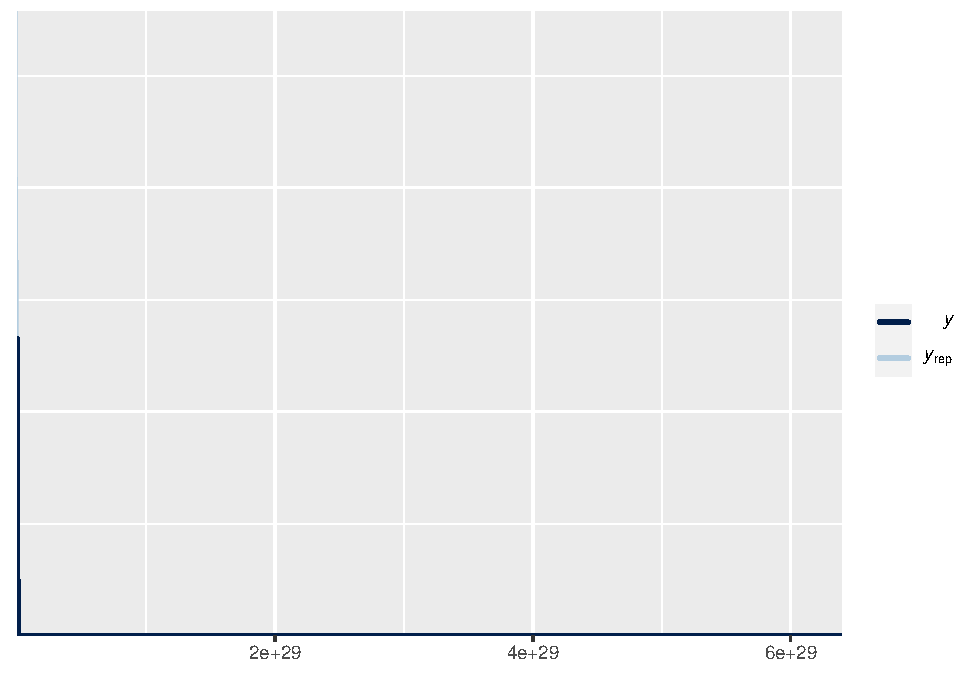
\includegraphics{assignment_1_final_files/figure-latex/unnamed-chunk-9-1.pdf}

\#\#\#fit the model

\begin{Shaded}
\begin{Highlighting}[]
\NormalTok{MLU\_prior\_m1\_fit }\OtherTok{\textless{}{-}} \FunctionTok{brm}\NormalTok{(}
\NormalTok{  MLU\_f1, }
  \AttributeTok{data =}\NormalTok{ sim\_data, }
  \AttributeTok{prior =}\NormalTok{ priors,}
  \AttributeTok{family =}\NormalTok{ lognorm\_fam,}
  \AttributeTok{refresh=}\DecValTok{0}\NormalTok{,}
  \AttributeTok{sample\_prior =} \ConstantTok{TRUE}\NormalTok{,}
  \AttributeTok{iter=}\DecValTok{6000}\NormalTok{,}
  \AttributeTok{warmup =} \DecValTok{2500}\NormalTok{,}
  \AttributeTok{backend =} \StringTok{"cmdstanr"}\NormalTok{,}
  \AttributeTok{threads =} \FunctionTok{threading}\NormalTok{(}\DecValTok{2}\NormalTok{),}
  \AttributeTok{chains =} \DecValTok{2}\NormalTok{,}
  \AttributeTok{cores =} \DecValTok{2}\NormalTok{,}
  \AttributeTok{control =} \FunctionTok{list}\NormalTok{(}
    \AttributeTok{adapt\_delta =} \FloatTok{0.99}\NormalTok{,}
    \AttributeTok{max\_treedepth =} \DecValTok{20}
\NormalTok{)}
\NormalTok{)}
\end{Highlighting}
\end{Shaded}

\#\#\#posterior predictive check

\begin{Shaded}
\begin{Highlighting}[]
\FunctionTok{pp\_check}\NormalTok{(MLU\_prior\_m1\_fit, }\AttributeTok{ndraws =} \DecValTok{100}\NormalTok{)}
\end{Highlighting}
\end{Shaded}

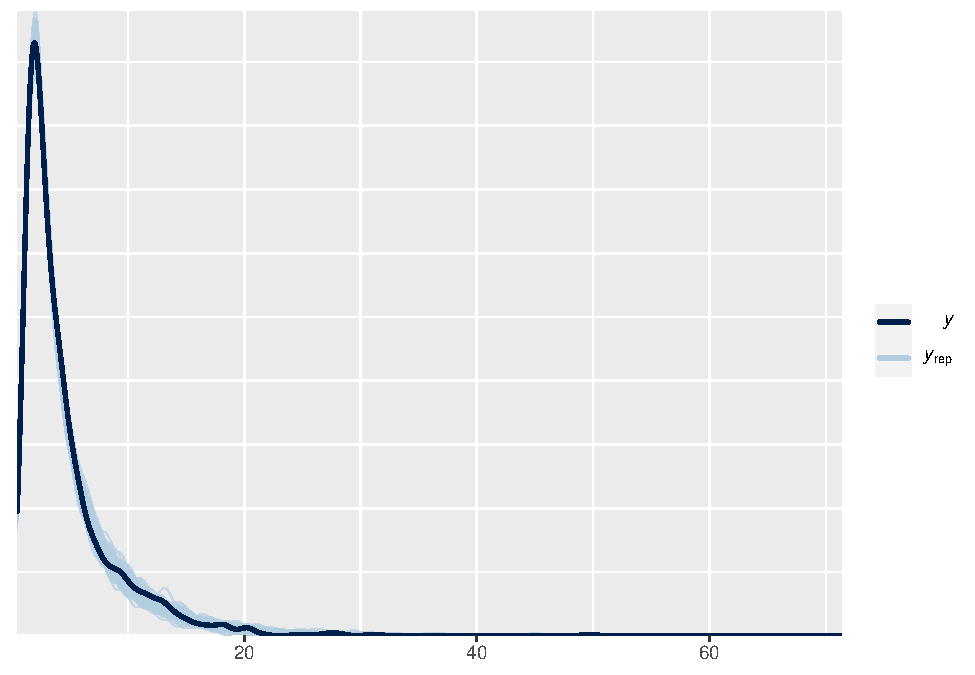
\includegraphics{assignment_1_final_files/figure-latex/unnamed-chunk-11-1.pdf}
\#\#\#traceplot for fitted model

\begin{Shaded}
\begin{Highlighting}[]
\FunctionTok{plot}\NormalTok{(MLU\_prior\_m1\_fit)}
\end{Highlighting}
\end{Shaded}

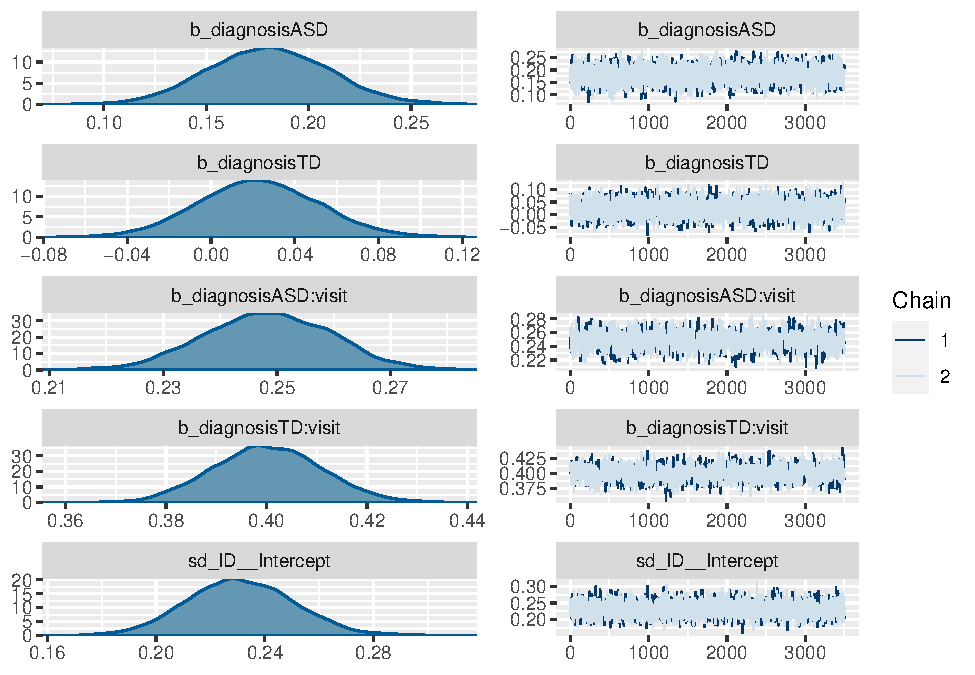
\includegraphics{assignment_1_final_files/figure-latex/unnamed-chunk-12-1.pdf}
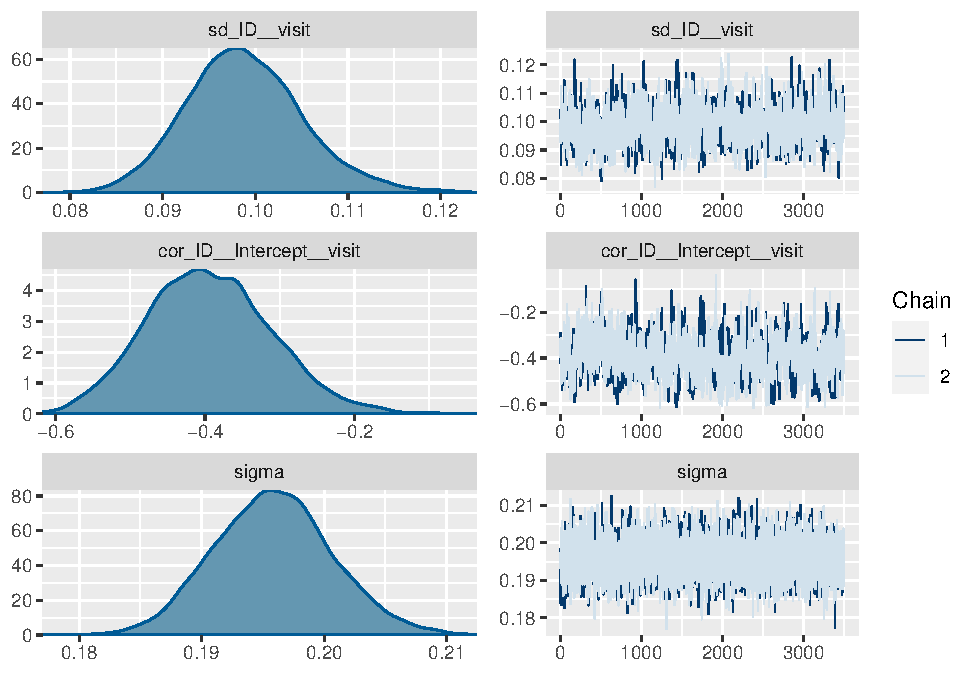
\includegraphics{assignment_1_final_files/figure-latex/unnamed-chunk-12-2.pdf}

Ditlev \#\#\# parameter recovery from fitted model

\begin{Shaded}
\begin{Highlighting}[]
\FunctionTok{print}\NormalTok{(MLU\_prior\_m1\_fit)}
\end{Highlighting}
\end{Shaded}

\begin{verbatim}
##  Family: lognormal 
##   Links: mu = identity; sigma = identity 
## Formula: MLU ~ 0 + diagnosis + diagnosis:visit + (1 + visit | ID) 
##    Data: sim_data (Number of observations: 1200) 
##   Draws: 2 chains, each with iter = 6000; warmup = 2500; thin = 1;
##          total post-warmup draws = 7000
## 
## Group-Level Effects: 
## ~ID (Number of levels: 200) 
##                      Estimate Est.Error l-95% CI u-95% CI Rhat Bulk_ESS
## sd(Intercept)            0.25      0.02     0.21     0.29 1.00     2913
## sd(visit)                0.10      0.01     0.09     0.11 1.00      775
## cor(Intercept,visit)    -0.38      0.08    -0.53    -0.22 1.01      426
##                      Tail_ESS
## sd(Intercept)            4857
## sd(visit)                1660
## cor(Intercept,visit)      798
## 
## Population-Level Effects: 
##                    Estimate Est.Error l-95% CI u-95% CI Rhat Bulk_ESS Tail_ESS
## diagnosisASD           0.14      0.03     0.08     0.20 1.00     3926     4188
## diagnosisTD            0.06      0.03     0.00     0.12 1.00     4183     5203
## diagnosisASD:visit     0.28      0.01     0.26     0.31 1.00     1321     2282
## diagnosisTD:visit      0.39      0.01     0.37     0.41 1.00     1085     2281
## 
## Family Specific Parameters: 
##       Estimate Est.Error l-95% CI u-95% CI Rhat Bulk_ESS Tail_ESS
## sigma     0.20      0.01     0.19     0.21 1.00     4332     5388
## 
## Draws were sampled using sample(hmc). For each parameter, Bulk_ESS
## and Tail_ESS are effective sample size measures, and Rhat is the potential
## scale reduction factor on split chains (at convergence, Rhat = 1).
\end{verbatim}

\hypertarget{prior-posterior-update-check}{%
\subsubsection{prior posterior update
check}\label{prior-posterior-update-check}}

\begin{Shaded}
\begin{Highlighting}[]
\NormalTok{posterior }\OtherTok{\textless{}{-}} \FunctionTok{as\_draws\_df}\NormalTok{(MLU\_prior\_m1\_fit)}

\NormalTok{plot1 }\OtherTok{\textless{}{-}} \FunctionTok{ggplot}\NormalTok{(posterior)}\SpecialCharTok{+}
  \FunctionTok{geom\_histogram}\NormalTok{(}\FunctionTok{aes}\NormalTok{(prior\_b\_diagnosisASD), }\AttributeTok{fill=}\StringTok{\textquotesingle{}red\textquotesingle{}}\NormalTok{, }\AttributeTok{color=}\StringTok{\textquotesingle{}black\textquotesingle{}}\NormalTok{, }\AttributeTok{alpha=}\FloatTok{0.3}\NormalTok{, }\AttributeTok{bins=}\DecValTok{50}\NormalTok{)}\SpecialCharTok{+}
  \FunctionTok{geom\_histogram}\NormalTok{(}\FunctionTok{aes}\NormalTok{(b\_diagnosisASD), }\AttributeTok{fill=}\StringTok{\textquotesingle{}green\textquotesingle{}}\NormalTok{, }\AttributeTok{color=}\StringTok{\textquotesingle{}black\textquotesingle{}}\NormalTok{, }\AttributeTok{alpha=}\FloatTok{0.3}\NormalTok{, }\AttributeTok{bins=}\DecValTok{50}\NormalTok{)}\SpecialCharTok{+}
  \FunctionTok{theme\_classic}\NormalTok{()}\SpecialCharTok{+}
  \FunctionTok{ggtitle}\NormalTok{(}\StringTok{\textquotesingle{}prior{-}posterior update check on interceps for ASD\textquotesingle{}}\NormalTok{)}\SpecialCharTok{+}
  \FunctionTok{xlab}\NormalTok{(}\StringTok{\textquotesingle{}intercept for ASD\textquotesingle{}}\NormalTok{)}

\NormalTok{plot2 }\OtherTok{\textless{}{-}} \FunctionTok{ggplot}\NormalTok{(posterior)}\SpecialCharTok{+}
  \FunctionTok{geom\_histogram}\NormalTok{(}\FunctionTok{aes}\NormalTok{(prior\_b\_diagnosisTD), }\AttributeTok{fill=}\StringTok{\textquotesingle{}red\textquotesingle{}}\NormalTok{, }\AttributeTok{color=}\StringTok{\textquotesingle{}black\textquotesingle{}}\NormalTok{, }\AttributeTok{alpha=}\FloatTok{0.3}\NormalTok{, }\AttributeTok{bins=}\DecValTok{50}\NormalTok{)}\SpecialCharTok{+}
  \FunctionTok{geom\_histogram}\NormalTok{(}\FunctionTok{aes}\NormalTok{(b\_diagnosisTD), }\AttributeTok{fill=}\StringTok{\textquotesingle{}green\textquotesingle{}}\NormalTok{, }\AttributeTok{color=}\StringTok{\textquotesingle{}black\textquotesingle{}}\NormalTok{, }\AttributeTok{alpha=}\FloatTok{0.3}\NormalTok{, }\AttributeTok{bins=}\DecValTok{50}\NormalTok{)}\SpecialCharTok{+}
  \FunctionTok{theme\_classic}\NormalTok{()}\SpecialCharTok{+}
  \FunctionTok{ggtitle}\NormalTok{(}\StringTok{\textquotesingle{}prior{-}posterior update check on intercept for TD\textquotesingle{}}\NormalTok{)}\SpecialCharTok{+}
  \FunctionTok{xlab}\NormalTok{(}\StringTok{\textquotesingle{}intercept for TD\textquotesingle{}}\NormalTok{)}

\NormalTok{plot3 }\OtherTok{\textless{}{-}} \FunctionTok{ggplot}\NormalTok{(posterior)}\SpecialCharTok{+}
  \FunctionTok{geom\_histogram}\NormalTok{(}\FunctionTok{aes}\NormalTok{(}\StringTok{\textasciigrave{}}\AttributeTok{prior\_b\_diagnosisASD:visit}\StringTok{\textasciigrave{}}\NormalTok{), }\AttributeTok{fill=}\StringTok{\textquotesingle{}red\textquotesingle{}}\NormalTok{, }\AttributeTok{color=}\StringTok{\textquotesingle{}black\textquotesingle{}}\NormalTok{, }\AttributeTok{alpha=}\FloatTok{0.3}\NormalTok{, }\AttributeTok{bins=}\DecValTok{50}\NormalTok{)}\SpecialCharTok{+}
  \FunctionTok{geom\_histogram}\NormalTok{(}\FunctionTok{aes}\NormalTok{(}\StringTok{\textasciigrave{}}\AttributeTok{b\_diagnosisASD:visit}\StringTok{\textasciigrave{}}\NormalTok{), }\AttributeTok{fill=}\StringTok{\textquotesingle{}green\textquotesingle{}}\NormalTok{, }\AttributeTok{color=}\StringTok{\textquotesingle{}black\textquotesingle{}}\NormalTok{, }\AttributeTok{alpha=}\FloatTok{0.3}\NormalTok{, }\AttributeTok{bins=}\DecValTok{50}\NormalTok{)}\SpecialCharTok{+}
  \FunctionTok{theme\_classic}\NormalTok{()}\SpecialCharTok{+}
  \FunctionTok{ggtitle}\NormalTok{(}\StringTok{\textquotesingle{}prior{-}posterior update check on slope for ASD\textquotesingle{}}\NormalTok{)}\SpecialCharTok{+}
  \FunctionTok{xlab}\NormalTok{(}\StringTok{"Slope for ASD"}\NormalTok{)}

\NormalTok{plot4 }\OtherTok{\textless{}{-}} \FunctionTok{ggplot}\NormalTok{(posterior)}\SpecialCharTok{+}
  \FunctionTok{geom\_histogram}\NormalTok{(}\FunctionTok{aes}\NormalTok{(}\StringTok{\textasciigrave{}}\AttributeTok{prior\_b\_diagnosisTD:visit}\StringTok{\textasciigrave{}}\NormalTok{), }\AttributeTok{fill=}\StringTok{\textquotesingle{}red\textquotesingle{}}\NormalTok{, }\AttributeTok{color=}\StringTok{\textquotesingle{}black\textquotesingle{}}\NormalTok{, }\AttributeTok{alpha=}\FloatTok{0.3}\NormalTok{, }\AttributeTok{bins=}\DecValTok{50}\NormalTok{)}\SpecialCharTok{+}
  \FunctionTok{geom\_histogram}\NormalTok{(}\FunctionTok{aes}\NormalTok{(}\StringTok{\textasciigrave{}}\AttributeTok{b\_diagnosisTD:visit}\StringTok{\textasciigrave{}}\NormalTok{), }\AttributeTok{fill=}\StringTok{\textquotesingle{}green\textquotesingle{}}\NormalTok{, }\AttributeTok{color=}\StringTok{\textquotesingle{}black\textquotesingle{}}\NormalTok{, }\AttributeTok{alpha=}\FloatTok{0.3}\NormalTok{, }\AttributeTok{bins=}\DecValTok{50}\NormalTok{)}\SpecialCharTok{+}
  \FunctionTok{theme\_classic}\NormalTok{()}\SpecialCharTok{+}
  \FunctionTok{ggtitle}\NormalTok{(}\StringTok{\textquotesingle{}prior{-}posterior update check on slope for TD\textquotesingle{}}\NormalTok{)}\SpecialCharTok{+}
  \FunctionTok{xlab}\NormalTok{(}\StringTok{"slope for TD"}\NormalTok{)}


\NormalTok{plot5 }\OtherTok{\textless{}{-}} \FunctionTok{ggplot}\NormalTok{(posterior)}\SpecialCharTok{+}
  \FunctionTok{geom\_histogram}\NormalTok{(}\FunctionTok{aes}\NormalTok{(prior\_cor\_ID), }\AttributeTok{fill=}\StringTok{\textquotesingle{}red\textquotesingle{}}\NormalTok{, }\AttributeTok{color=}\StringTok{\textquotesingle{}black\textquotesingle{}}\NormalTok{, }\AttributeTok{alpha=}\FloatTok{0.3}\NormalTok{, }\AttributeTok{bins=}\DecValTok{50}\NormalTok{)}\SpecialCharTok{+}
  \FunctionTok{geom\_histogram}\NormalTok{(}\FunctionTok{aes}\NormalTok{(cor\_ID\_\_Intercept\_\_visit), }\AttributeTok{fill=}\StringTok{\textquotesingle{}green\textquotesingle{}}\NormalTok{, }\AttributeTok{color=}\StringTok{\textquotesingle{}black\textquotesingle{}}\NormalTok{, }\AttributeTok{alpha=}\FloatTok{0.3}\NormalTok{, }\AttributeTok{bins=}\DecValTok{50}\NormalTok{)}\SpecialCharTok{+}
  \FunctionTok{theme\_classic}\NormalTok{()}\SpecialCharTok{+}
  \FunctionTok{ggtitle}\NormalTok{(}\StringTok{\textquotesingle{}prior{-}posterior update check on correlation between varying intercepts and slopes\textquotesingle{}}\NormalTok{)}\SpecialCharTok{+}
  \FunctionTok{xlab}\NormalTok{(}\StringTok{"Correlation"}\NormalTok{)}

\NormalTok{plot6 }\OtherTok{\textless{}{-}} \FunctionTok{ggplot}\NormalTok{(posterior)}\SpecialCharTok{+}
  \FunctionTok{geom\_histogram}\NormalTok{(}\FunctionTok{aes}\NormalTok{(prior\_sd\_ID), }\AttributeTok{fill=}\StringTok{\textquotesingle{}red\textquotesingle{}}\NormalTok{, }\AttributeTok{color=}\StringTok{\textquotesingle{}black\textquotesingle{}}\NormalTok{, }\AttributeTok{alpha=}\FloatTok{0.3}\NormalTok{, }\AttributeTok{bins=}\DecValTok{50}\NormalTok{)}\SpecialCharTok{+}
  \FunctionTok{geom\_histogram}\NormalTok{(}\FunctionTok{aes}\NormalTok{(sd\_ID\_\_Intercept), }\AttributeTok{fill=}\StringTok{\textquotesingle{}green\textquotesingle{}}\NormalTok{, }\AttributeTok{color=}\StringTok{\textquotesingle{}black\textquotesingle{}}\NormalTok{, }\AttributeTok{alpha=}\FloatTok{0.3}\NormalTok{, }\AttributeTok{bins=}\DecValTok{50}\NormalTok{)}\SpecialCharTok{+}
  \FunctionTok{theme\_classic}\NormalTok{()}\SpecialCharTok{+}
  \FunctionTok{ggtitle}\NormalTok{(}\StringTok{\textquotesingle{}Prior{-}posterior update check, the variability of the intercept\textquotesingle{}}\NormalTok{)}\SpecialCharTok{+}
  \FunctionTok{xlab}\NormalTok{(}\StringTok{"Intercept"}\NormalTok{)}

\NormalTok{plot7 }\OtherTok{\textless{}{-}} \FunctionTok{ggplot}\NormalTok{(posterior)}\SpecialCharTok{+}
  \FunctionTok{geom\_histogram}\NormalTok{(}\FunctionTok{aes}\NormalTok{(prior\_sd\_ID), }\AttributeTok{fill=}\StringTok{\textquotesingle{}red\textquotesingle{}}\NormalTok{, }\AttributeTok{color=}\StringTok{\textquotesingle{}black\textquotesingle{}}\NormalTok{, }\AttributeTok{alpha=}\FloatTok{0.3}\NormalTok{, }\AttributeTok{bins=}\DecValTok{50}\NormalTok{)}\SpecialCharTok{+}
  \FunctionTok{geom\_histogram}\NormalTok{(}\FunctionTok{aes}\NormalTok{(sd\_ID\_\_visit), }\AttributeTok{fill=}\StringTok{\textquotesingle{}green\textquotesingle{}}\NormalTok{, }\AttributeTok{color=}\StringTok{\textquotesingle{}black\textquotesingle{}}\NormalTok{, }\AttributeTok{alpha=}\FloatTok{0.3}\NormalTok{, }\AttributeTok{bins=}\DecValTok{50}\NormalTok{)}\SpecialCharTok{+}
  \FunctionTok{theme\_classic}\NormalTok{()}\SpecialCharTok{+}
  \FunctionTok{ggtitle}\NormalTok{(}\StringTok{\textquotesingle{}Prior{-}posterior update check, the variability of the slopes\textquotesingle{}}\NormalTok{)}\SpecialCharTok{+}
  \FunctionTok{xlab}\NormalTok{(}\StringTok{"Intercept"}\NormalTok{)}


\NormalTok{plot1}
\end{Highlighting}
\end{Shaded}

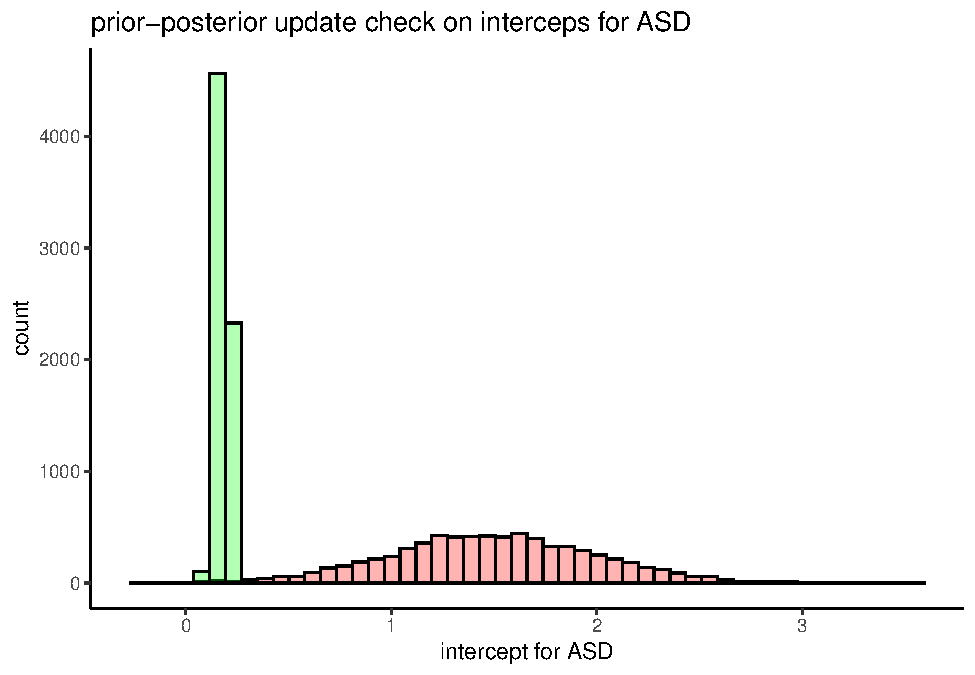
\includegraphics{assignment_1_final_files/figure-latex/unnamed-chunk-14-1.pdf}

\begin{Shaded}
\begin{Highlighting}[]
\NormalTok{plot2}
\end{Highlighting}
\end{Shaded}

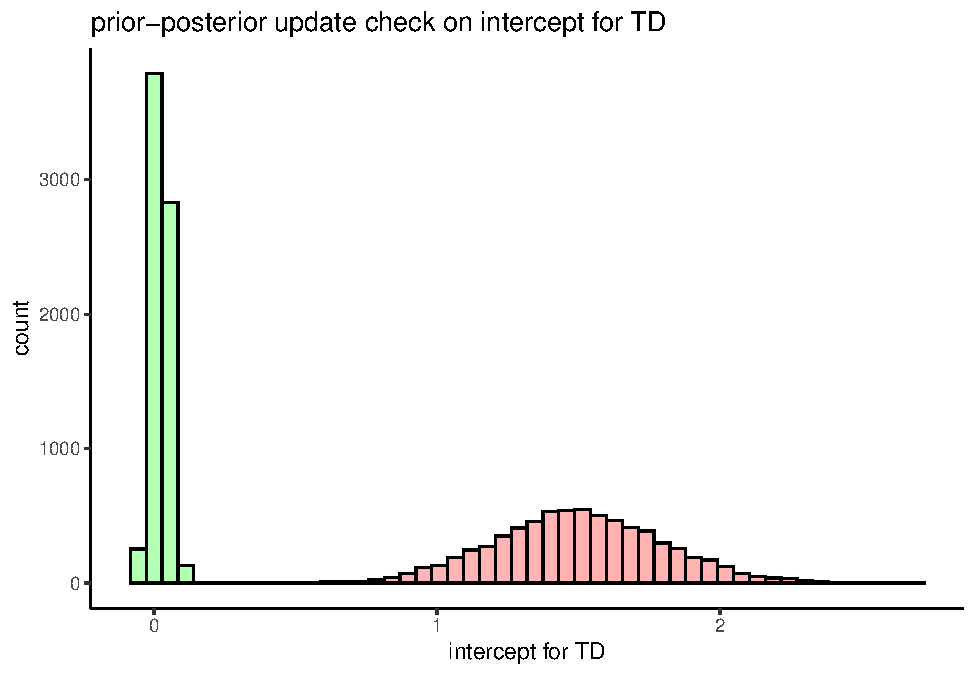
\includegraphics{assignment_1_final_files/figure-latex/unnamed-chunk-14-2.pdf}

\begin{Shaded}
\begin{Highlighting}[]
\NormalTok{plot3}
\end{Highlighting}
\end{Shaded}

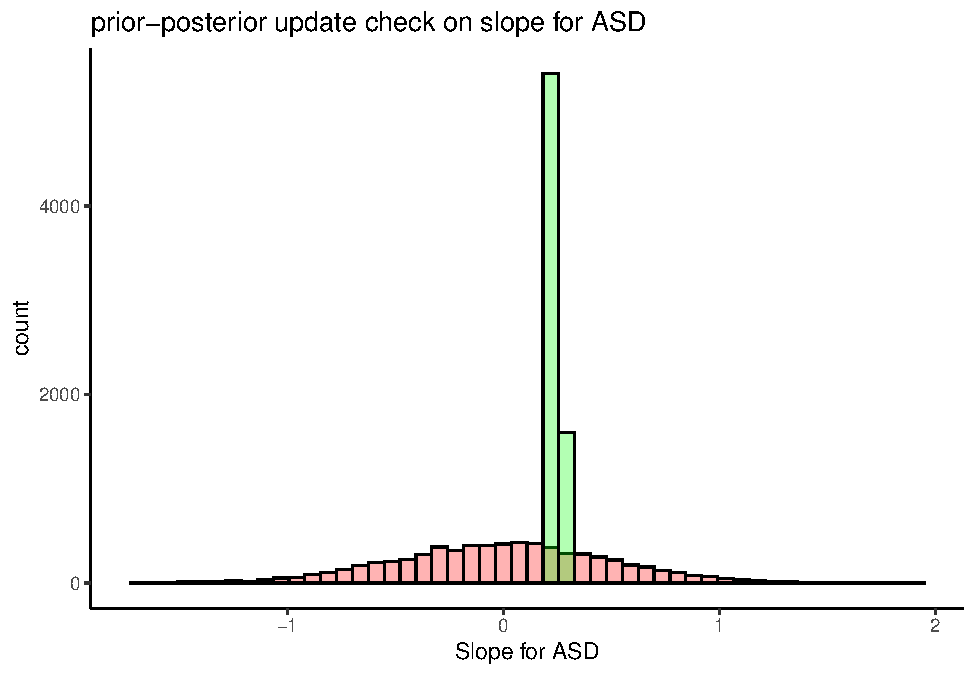
\includegraphics{assignment_1_final_files/figure-latex/unnamed-chunk-14-3.pdf}

\begin{Shaded}
\begin{Highlighting}[]
\NormalTok{plot4}
\end{Highlighting}
\end{Shaded}

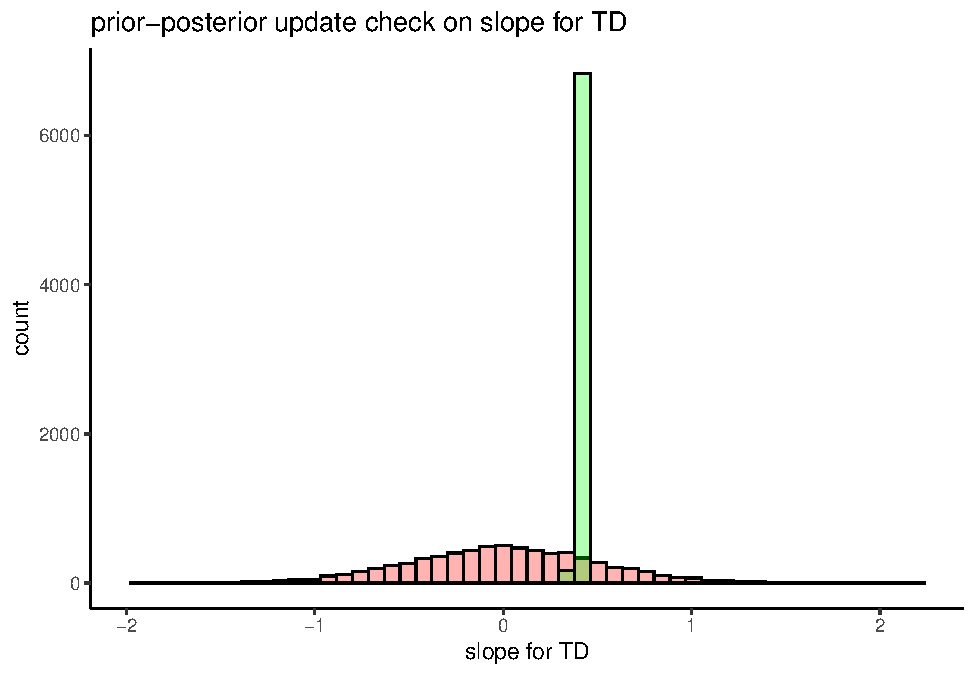
\includegraphics{assignment_1_final_files/figure-latex/unnamed-chunk-14-4.pdf}

\begin{Shaded}
\begin{Highlighting}[]
\NormalTok{plot5}
\end{Highlighting}
\end{Shaded}

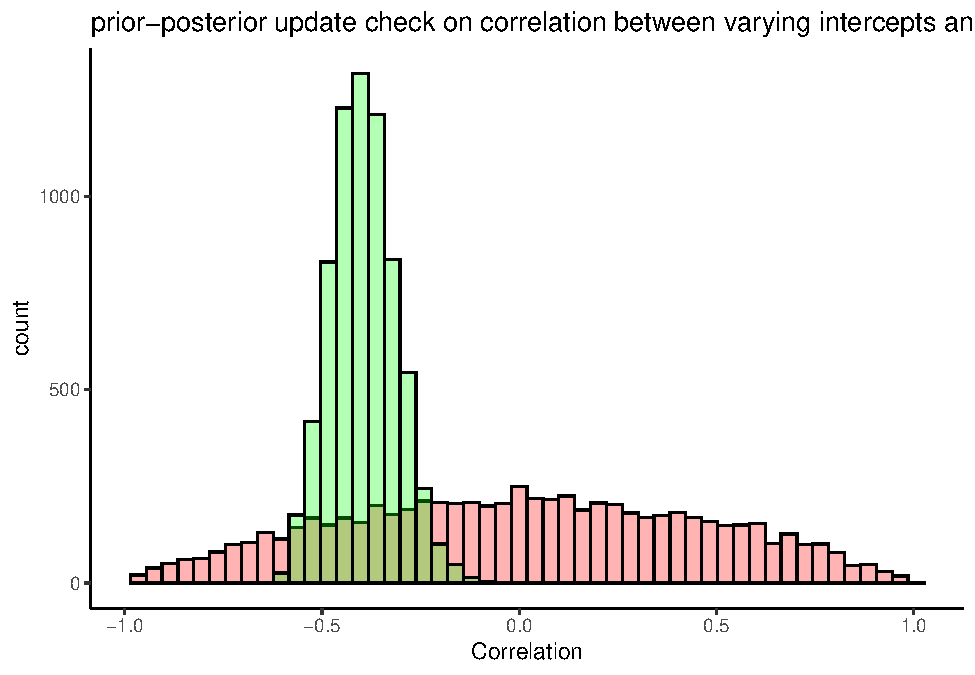
\includegraphics{assignment_1_final_files/figure-latex/unnamed-chunk-14-5.pdf}

\begin{Shaded}
\begin{Highlighting}[]
\NormalTok{plot6}
\end{Highlighting}
\end{Shaded}

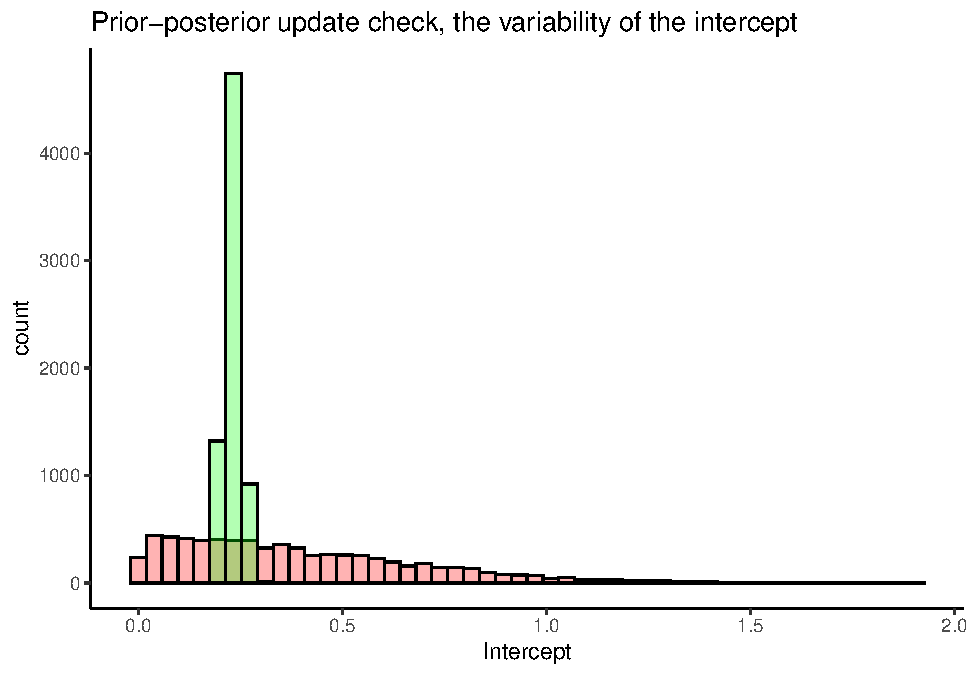
\includegraphics{assignment_1_final_files/figure-latex/unnamed-chunk-14-6.pdf}

\begin{Shaded}
\begin{Highlighting}[]
\NormalTok{plot7}
\end{Highlighting}
\end{Shaded}

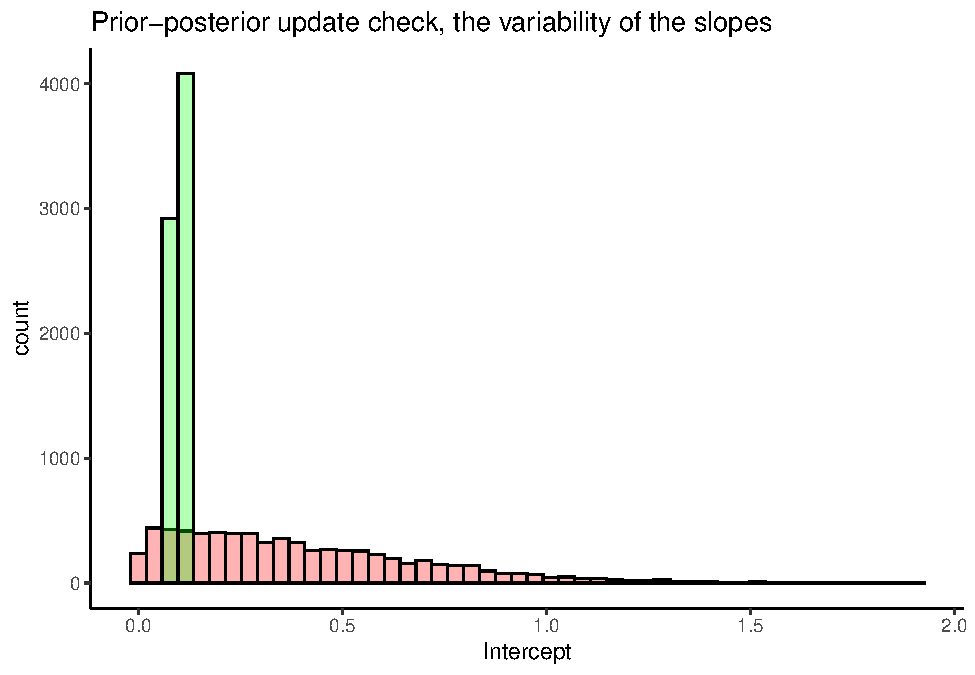
\includegraphics{assignment_1_final_files/figure-latex/unnamed-chunk-14-7.pdf}

\hypertarget{estimating-effectsize-baysian-power-analysis}{%
\subsubsection{Estimating effectsize, baysian power
analysis}\label{estimating-effectsize-baysian-power-analysis}}

\hypertarget{function-simulates-data-and-return-ci-of-slope-difference}{%
\paragraph{Function simulates data and return CI of slope
difference}\label{function-simulates-data-and-return-ci-of-slope-difference}}

\begin{Shaded}
\begin{Highlighting}[]
\NormalTok{ fun\_sim\_data }\OtherTok{\textless{}{-}} \ControlFlowTok{function}\NormalTok{(seed,n)\{}
   \FunctionTok{set.seed}\NormalTok{(seed)}
   
\NormalTok{   average\_mlu }\OtherTok{\textless{}{-}} \FunctionTok{log}\NormalTok{(}\FloatTok{1.5}\NormalTok{)}
\NormalTok{ sd\_mlu\_asd }\OtherTok{\textless{}{-}} \FunctionTok{log}\NormalTok{(}\FloatTok{1.5+0.5}\NormalTok{)}\SpecialCharTok{{-}}\FunctionTok{log}\NormalTok{(}\FloatTok{1.5}\NormalTok{)}
\NormalTok{ sd\_mlu\_td }\OtherTok{\textless{}{-}} \FunctionTok{log}\NormalTok{(}\FloatTok{1.5+0.3}\NormalTok{)}\SpecialCharTok{{-}}\FunctionTok{log}\NormalTok{(}\FloatTok{1.5}\NormalTok{)}
 
\NormalTok{ change\_mlu\_asd }\OtherTok{\textless{}{-}} \FloatTok{0.4}\SpecialCharTok{/}\FloatTok{1.5}
\NormalTok{ change\_mlu\_td }\OtherTok{\textless{}{-}} \FloatTok{0.6}\SpecialCharTok{/}\FloatTok{1.5}
\NormalTok{ change\_sd\_mlu\_asd }\OtherTok{\textless{}{-}} \FloatTok{0.4}\SpecialCharTok{*}\NormalTok{(}\FloatTok{0.4}\SpecialCharTok{/}\FloatTok{1.5}\NormalTok{)}
\NormalTok{ change\_sd\_mlu\_td }\OtherTok{\textless{}{-}} \FloatTok{0.2}\SpecialCharTok{*}\NormalTok{(}\FloatTok{0.6}\SpecialCharTok{/}\FloatTok{1.5}\NormalTok{)}
\NormalTok{ e }\OtherTok{\textless{}{-}} \FloatTok{0.2}
 
\NormalTok{ int\_asd }\OtherTok{\textless{}{-}} \FunctionTok{rnorm}\NormalTok{(n, }\AttributeTok{mean=}\NormalTok{average\_mlu, }\AttributeTok{sd=}\NormalTok{sd\_mlu\_asd)}
\NormalTok{int\_td }\OtherTok{\textless{}{-}} \FunctionTok{rnorm}\NormalTok{(n, }\AttributeTok{mean=}\NormalTok{average\_mlu, }\AttributeTok{sd=}\NormalTok{sd\_mlu\_td)}

\NormalTok{slope\_asd }\OtherTok{\textless{}{-}} \FunctionTok{rnorm}\NormalTok{(n, }\AttributeTok{mean=}\NormalTok{change\_mlu\_asd, }\AttributeTok{sd=}\NormalTok{change\_sd\_mlu\_asd)}
\NormalTok{slope\_td }\OtherTok{\textless{}{-}} \FunctionTok{rnorm}\NormalTok{(n, }\AttributeTok{mean =}\NormalTok{ change\_mlu\_td, }\AttributeTok{sd=}\NormalTok{change\_sd\_mlu\_td)}



\NormalTok{   data }\OtherTok{\textless{}{-}} 
     \FunctionTok{tibble}\NormalTok{(}\AttributeTok{diagnosis=}\FunctionTok{rep}\NormalTok{(}\FunctionTok{c}\NormalTok{(}\StringTok{\textquotesingle{}TD\textquotesingle{}}\NormalTok{, }\StringTok{\textquotesingle{}ASD\textquotesingle{}}\NormalTok{), }\AttributeTok{each=}\NormalTok{n)) }\SpecialCharTok{\%\textgreater{}\%} 
     \FunctionTok{mutate}\NormalTok{(}\AttributeTok{intercept=}\FunctionTok{ifelse}\NormalTok{(diagnosis}\SpecialCharTok{==}\StringTok{\textquotesingle{}TD\textquotesingle{}}\NormalTok{, int\_td, int\_asd)) }\SpecialCharTok{\%\textgreater{}\%} 

     \FunctionTok{mutate}\NormalTok{(}\AttributeTok{slope=}\FunctionTok{ifelse}\NormalTok{(diagnosis}\SpecialCharTok{==}\StringTok{\textquotesingle{}TD\textquotesingle{}}\NormalTok{, slope\_td, slope\_asd)) }\SpecialCharTok{\%\textgreater{}\%} 
     \FunctionTok{mutate}\NormalTok{(}\AttributeTok{error=}\FunctionTok{ifelse}\NormalTok{(diagnosis}\SpecialCharTok{==}\StringTok{\textquotesingle{}TD\textquotesingle{}}\NormalTok{, e, e)) }\SpecialCharTok{\%\textgreater{}\%} 
\NormalTok{     dplyr}\SpecialCharTok{::}\FunctionTok{mutate}\NormalTok{(}\AttributeTok{ID=}\FunctionTok{row\_number}\NormalTok{()) }\SpecialCharTok{\%\textgreater{}\%} 
     \FunctionTok{slice}\NormalTok{(}\FunctionTok{rep}\NormalTok{(}\DecValTok{1}\SpecialCharTok{:}\FunctionTok{n}\NormalTok{(), }\AttributeTok{each=}\DecValTok{6}\NormalTok{)) }\SpecialCharTok{\%\textgreater{}\%} 
     \FunctionTok{add\_column}\NormalTok{(}\AttributeTok{visit=}\FunctionTok{rep}\NormalTok{(}\FunctionTok{c}\NormalTok{(}\DecValTok{1}\NormalTok{,}\DecValTok{2}\NormalTok{,}\DecValTok{3}\NormalTok{,}\DecValTok{4}\NormalTok{,}\DecValTok{5}\NormalTok{,}\DecValTok{6}\NormalTok{), }\AttributeTok{times=}\NormalTok{n}\SpecialCharTok{+}\NormalTok{n))}
 
 \ControlFlowTok{for}\NormalTok{(i }\ControlFlowTok{in} \FunctionTok{seq}\NormalTok{(}\FunctionTok{nrow}\NormalTok{(data)))\{}
\NormalTok{   data}\SpecialCharTok{$}\NormalTok{MLU[i] }\OtherTok{\textless{}{-}} \FunctionTok{exp}\NormalTok{(}\FunctionTok{rnorm}\NormalTok{(}\DecValTok{1}\NormalTok{,data}\SpecialCharTok{$}\NormalTok{intercept[i]}\SpecialCharTok{+}\NormalTok{(data}\SpecialCharTok{$}\NormalTok{slope[i]}\SpecialCharTok{*}\NormalTok{(data}\SpecialCharTok{$}\NormalTok{visit[i]}\SpecialCharTok{{-}}\DecValTok{1}\NormalTok{)), data}\SpecialCharTok{$}\NormalTok{error[i]))}
\NormalTok{ \}}
\NormalTok{   data }\OtherTok{\textless{}{-}}\NormalTok{ data[,}\FunctionTok{c}\NormalTok{(}\DecValTok{1}\NormalTok{,}\DecValTok{5}\NormalTok{,}\DecValTok{6}\NormalTok{,}\DecValTok{2}\NormalTok{,}\DecValTok{3}\NormalTok{,}\DecValTok{4}\NormalTok{,}\DecValTok{7}\NormalTok{)]}
\NormalTok{   post }\OtherTok{\textless{}{-}} \FunctionTok{update}\NormalTok{(MLU\_prior\_m1\_fit,}
                  \AttributeTok{newdata =}\NormalTok{ data,}
                  \AttributeTok{seed=}\NormalTok{seed) }\SpecialCharTok{\%\textgreater{}\%} 
     \FunctionTok{as\_draws\_df}\NormalTok{() }\SpecialCharTok{\%\textgreater{}\%} 
     \FunctionTok{mutate}\NormalTok{(}\AttributeTok{slope\_diff=}\NormalTok{(}\StringTok{\textasciigrave{}}\AttributeTok{b\_diagnosisTD:visit}\StringTok{\textasciigrave{}}\SpecialCharTok{{-}} \StringTok{\textasciigrave{}}\AttributeTok{b\_diagnosisASD:visit}\StringTok{\textasciigrave{}}\NormalTok{))}
   
\NormalTok{   CI }\OtherTok{\textless{}{-}} \FunctionTok{as.data.frame}\NormalTok{(}\FunctionTok{t}\NormalTok{(}\FunctionTok{quantile}\NormalTok{(post}\SpecialCharTok{$}\NormalTok{slope\_diff, }\AttributeTok{probs=}\FunctionTok{c}\NormalTok{(}\FloatTok{0.025}\NormalTok{, }\FloatTok{0.975}\NormalTok{)))) }\SpecialCharTok{\%\textgreater{}\%} 
     \FunctionTok{add\_column}\NormalTok{(}\AttributeTok{mean=}\FunctionTok{mean}\NormalTok{(post}\SpecialCharTok{$}\NormalTok{slope\_diff))}
   \FunctionTok{return}\NormalTok{(CI)\}}
\end{Highlighting}
\end{Shaded}

Manuela \#\#\#\# running the functiong with different amount of
participants

\begin{Shaded}
\begin{Highlighting}[]
\CommentTok{\# n\_sim \textless{}{-} 10}
\CommentTok{\# }
\CommentTok{\# s10 \textless{}{-} tibble(seed=1:n\_sim) \%\textgreater{}\% }
\CommentTok{\#   mutate(b1=purrr::map(seed, fun\_sim\_data, n=10)) \%\textgreater{}\% }
\CommentTok{\#   unnest(b1)}
\CommentTok{\# }
\CommentTok{\# s15 \textless{}{-} tibble(seed=1:n\_sim) \%\textgreater{}\% }
\CommentTok{\#   mutate(b1=purrr::map(seed, fun\_sim\_data, n=15)) \%\textgreater{}\% }
\CommentTok{\#   unnest(b1)}
\CommentTok{\# }
\CommentTok{\# s20 \textless{}{-} tibble(seed=1:n\_sim) \%\textgreater{}\% }
\CommentTok{\#   mutate(b1=purrr::map(seed, fun\_sim\_data, n=20)) \%\textgreater{}\% }
\CommentTok{\#   unnest(b1)}
\CommentTok{\# }
\CommentTok{\# s30 \textless{}{-} tibble(seed=1:n\_sim) \%\textgreater{}\% }
\CommentTok{\#   mutate(b1=purrr::map(seed, fun\_sim\_data, n=30)) \%\textgreater{}\% }
\CommentTok{\#   unnest(b1)}
\CommentTok{\# }
\CommentTok{\# s40 \textless{}{-} tibble(seed=1:n\_sim) \%\textgreater{}\% }
\CommentTok{\#   mutate(b1=purrr::map(seed, fun\_sim\_data, n=40)) \%\textgreater{}\% }
\CommentTok{\#   unnest(b1)}
\CommentTok{\# }
\CommentTok{\# s50 \textless{}{-} tibble(seed=1:n\_sim) \%\textgreater{}\% }
\CommentTok{\#   mutate(b1=purrr::map(seed, fun\_sim\_data, n=50)) \%\textgreater{}\% }
\CommentTok{\#   unnest(b1)}
\CommentTok{\# }
\CommentTok{\# s75 \textless{}{-} tibble(seed=1:n\_sim) \%\textgreater{}\% }
\CommentTok{\#   mutate(b1=purrr::map(seed, fun\_sim\_data, n=75)) \%\textgreater{}\% }
\CommentTok{\#   unnest(b1)}
\CommentTok{\# }
\CommentTok{\# s100 \textless{}{-} tibble(seed=1:n\_sim) \%\textgreater{}\% }
\CommentTok{\#   mutate(b1=purrr::map(seed, fun\_sim\_data, n=100)) \%\textgreater{}\% }
\CommentTok{\#   unnest(b1)}
\CommentTok{\# }
\CommentTok{\# s180 \textless{}{-} tibble(seed=1:n\_sim) \%\textgreater{}\% }
\CommentTok{\#   mutate(b1=purrr::map(seed, fun\_sim\_data, n=180)) \%\textgreater{}\% }
\CommentTok{\#   unnest(b1)}
\CommentTok{\# }
\CommentTok{\# s250 \textless{}{-} tibble(seed=1:n\_sim) \%\textgreater{}\% }
\CommentTok{\#   mutate(b1=purrr::map(seed, fun\_sim\_data, n=250)) \%\textgreater{}\% }
\CommentTok{\#   unnest(b1)}
\CommentTok{\# }
\CommentTok{\# s300 \textless{}{-} tibble(seed=1:n\_sim) \%\textgreater{}\% }
\CommentTok{\#   mutate(b1=purrr::map(seed, fun\_sim\_data, n=300)) \%\textgreater{}\% }
\CommentTok{\#   unnest(b1)}
\end{Highlighting}
\end{Shaded}

\hypertarget{effectsize-of-slope-difference-plots}{%
\paragraph{Effectsize of slope difference
(plots)}\label{effectsize-of-slope-difference-plots}}

\begin{Shaded}
\begin{Highlighting}[]
\CommentTok{\# plot\_s10 \textless{}{-} s10 \%\textgreater{}\% }
\CommentTok{\#   ggplot(aes(x=seed, y=mean, ymin = \textasciigrave{}2.5\%\textasciigrave{}, ymax= \textasciigrave{}97.5\%\textasciigrave{} ))+}
\CommentTok{\#   geom\_pointrange(fatten = 1/2)+}
\CommentTok{\#   geom\_hline(yintercept = c(0, 0.5), colour= \textquotesingle{}green\textquotesingle{})+}
\CommentTok{\#   labs(x="seed (simulation index)", y= "slope difference")+}
\CommentTok{\#   ggtitle("slope difference, 10 participants")}
\CommentTok{\# }
\CommentTok{\# plot\_s15 \textless{}{-} s15 \%\textgreater{}\% }
\CommentTok{\#   ggplot(aes(x=seed, y=mean, ymin = \textasciigrave{}2.5\%\textasciigrave{}, ymax= \textasciigrave{}97.5\%\textasciigrave{} ))+}
\CommentTok{\#   geom\_pointrange(fatten = 1/2)+}
\CommentTok{\#   geom\_hline(yintercept = c(0, 0.5), colour= \textquotesingle{}green\textquotesingle{})+}
\CommentTok{\#   labs(x="seed (simulation index)", y= "slope difference")+}
\CommentTok{\#   ggtitle("slope difference, 15 participants")}
\CommentTok{\# }
\CommentTok{\# plot\_s20 \textless{}{-} s20 \%\textgreater{}\% }
\CommentTok{\#   ggplot(aes(x=seed, y=mean, ymin = \textasciigrave{}2.5\%\textasciigrave{}, ymax= \textasciigrave{}97.5\%\textasciigrave{} ))+}
\CommentTok{\#   geom\_pointrange(fatten = 1/2)+}
\CommentTok{\#   geom\_hline(yintercept = c(0, 0.5), colour= \textquotesingle{}green\textquotesingle{})+}
\CommentTok{\#   labs(x="seed (simulation index)", y= "slope difference")+}
\CommentTok{\#   ggtitle("slope difference, 20 participants")}
\CommentTok{\# }
\CommentTok{\# plot\_s30 \textless{}{-} s30 \%\textgreater{}\% }
\CommentTok{\#   ggplot(aes(x=seed, y=mean, ymin = \textasciigrave{}2.5\%\textasciigrave{}, ymax= \textasciigrave{}97.5\%\textasciigrave{} ))+}
\CommentTok{\#   geom\_pointrange(fatten = 1/2)+}
\CommentTok{\#   geom\_hline(yintercept = c(0, 0.5), colour= \textquotesingle{}green\textquotesingle{})+}
\CommentTok{\#   labs(x="seed (simulation index)", y= "slope difference")+}
\CommentTok{\#   ggtitle("slope difference, 30 participants")}
\CommentTok{\# }
\CommentTok{\# plot\_s40 \textless{}{-} s40 \%\textgreater{}\% }
\CommentTok{\#   ggplot(aes(x=seed, y=mean, ymin = \textasciigrave{}2.5\%\textasciigrave{}, ymax= \textasciigrave{}97.5\%\textasciigrave{} ))+}
\CommentTok{\#   geom\_pointrange(fatten = 1/2)+}
\CommentTok{\#   geom\_hline(yintercept = c(0, 0.5), colour= \textquotesingle{}green\textquotesingle{})+}
\CommentTok{\#   labs(x="seed (simulation index)", y= "slope difference")+}
\CommentTok{\#   ggtitle("slope difference, 40 participants")}
\CommentTok{\# }
\CommentTok{\# plot\_s50 \textless{}{-} s50 \%\textgreater{}\% }
\CommentTok{\#   ggplot(aes(x=seed, y=mean, ymin = \textasciigrave{}2.5\%\textasciigrave{}, ymax= \textasciigrave{}97.5\%\textasciigrave{} ))+}
\CommentTok{\#   geom\_pointrange(fatten = 1/2)+}
\CommentTok{\#   geom\_hline(yintercept = c(0, 0.5), colour= \textquotesingle{}green\textquotesingle{})+}
\CommentTok{\#   labs(x="seed (simulation index)", y= "slope difference")+}
\CommentTok{\#   ggtitle("slope difference, 50 participants")}
\CommentTok{\# }
\CommentTok{\# plot\_s75 \textless{}{-} s75 \%\textgreater{}\% }
\CommentTok{\#   ggplot(aes(x=seed, y=mean, ymin = \textasciigrave{}2.5\%\textasciigrave{}, ymax= \textasciigrave{}97.5\%\textasciigrave{} ))+}
\CommentTok{\#   geom\_pointrange(fatten = 1/2)+}
\CommentTok{\#   geom\_hline(yintercept = c(0, 0.5), colour= \textquotesingle{}green\textquotesingle{})+}
\CommentTok{\#   labs(x="seed (simulation index)", y= "slope difference")+}
\CommentTok{\#   ggtitle("slope difference, 75 participants")}
\CommentTok{\# }
\CommentTok{\# plot\_s100 \textless{}{-} s100 \%\textgreater{}\% }
\CommentTok{\#   ggplot(aes(x=seed, y=mean, ymin = \textasciigrave{}2.5\%\textasciigrave{}, ymax= \textasciigrave{}97.5\%\textasciigrave{} ))+}
\CommentTok{\#   geom\_pointrange(fatten = 1/2)+}
\CommentTok{\#   geom\_hline(yintercept = c(0, 0.5), colour= \textquotesingle{}green\textquotesingle{})+}
\CommentTok{\#   labs(x="seed (simulation index)", y= "slope difference")+}
\CommentTok{\#   ggtitle("slope difference, 100 participants")}
\CommentTok{\# }
\CommentTok{\# plot\_s180 \textless{}{-} s180 \%\textgreater{}\% }
\CommentTok{\#   ggplot(aes(x=seed, y=mean, ymin = \textasciigrave{}2.5\%\textasciigrave{}, ymax= \textasciigrave{}97.5\%\textasciigrave{} ))+}
\CommentTok{\#   geom\_pointrange(fatten = 1/2)+}
\CommentTok{\#   geom\_hline(yintercept = c(0, 0.5), colour= \textquotesingle{}green\textquotesingle{})+}
\CommentTok{\#   labs(x="seed (simulation index)", y= "slope difference")+}
\CommentTok{\#   ggtitle("slope difference, 180 participants")}
\CommentTok{\#   }
\CommentTok{\# plot\_s250 \textless{}{-} s250 \%\textgreater{}\% }
\CommentTok{\#   ggplot(aes(x=seed, y=mean, ymin = \textasciigrave{}2.5\%\textasciigrave{}, ymax= \textasciigrave{}97.5\%\textasciigrave{} ))+}
\CommentTok{\#   geom\_pointrange(fatten = 1/2)+}
\CommentTok{\#   geom\_hline(yintercept = c(0, 0.5), colour= \textquotesingle{}green\textquotesingle{})+}
\CommentTok{\#   labs(x="seed (simulation index)", y= "slope difference")+}
\CommentTok{\#   ggtitle("slope difference, 150 participants")}
\CommentTok{\# }
\CommentTok{\# plot\_s300 \textless{}{-} s300 \%\textgreater{}\% }
\CommentTok{\#   ggplot(aes(x=seed, y=mean, ymin = \textasciigrave{}2.5\%\textasciigrave{}, ymax= \textasciigrave{}97.5\%\textasciigrave{} ))+}
\CommentTok{\#   geom\_pointrange(fatten = 1/2)+}
\CommentTok{\#   geom\_hline(yintercept = c(0, 0.5), colour= \textquotesingle{}green\textquotesingle{})+}
\CommentTok{\#   labs(x="seed (simulation index)", y= "slope difference")+}
\CommentTok{\#   ggtitle("slope difference, 300 participants")}
\CommentTok{\# }
\CommentTok{\# grid.arrange(}
\CommentTok{\#   plot\_s10,}
\CommentTok{\#   plot\_s15,}
\CommentTok{\#   plot\_s20,}
\CommentTok{\#   plot\_s30,}
\CommentTok{\#   plot\_s40)}
\CommentTok{\# grid.arrange(}
\CommentTok{\#   plot\_s50,}
\CommentTok{\#   plot\_s75,}
\CommentTok{\#   plot\_s100,}
\CommentTok{\#   plot\_s180,}
\CommentTok{\#   plot\_s250,}
\CommentTok{\#   plot\_s300)}
\end{Highlighting}
\end{Shaded}

Patrik \#\#\#\# Power analysis

\begin{Shaded}
\begin{Highlighting}[]
\CommentTok{\# power\_analysis\_fun \textless{}{-} function(sim\_nr, n)\{}
\CommentTok{\#   sim\_nr \%\textgreater{}\% }
\CommentTok{\#     mutate(two\_half=ifelse(\textasciigrave{}2.5\%\textasciigrave{}\textgreater{}0,1,0 )) \%\textgreater{}\%}
\CommentTok{\#     summarise(power=mean(two\_half)) \%\textgreater{}\% }
\CommentTok{\#     add\_column(number\_of\_participants=n)}
\CommentTok{\# \}}
\CommentTok{\# }
\CommentTok{\# power\_analysis\_sum \textless{}{-} bind\_rows(}
\CommentTok{\#   power\_analysis\_fun(s10, 10),}
\CommentTok{\#   power\_analysis\_fun(s15, 15),}
\CommentTok{\#   power\_analysis\_fun(s20, 20),}
\CommentTok{\#   power\_analysis\_fun(s30, 30),}
\CommentTok{\#   power\_analysis\_fun(s40, 40),}
\CommentTok{\#   power\_analysis\_fun(s50, 50),}
\CommentTok{\#   power\_analysis\_fun(s75, 75),}
\CommentTok{\#   power\_analysis\_fun(s100, 100),}
\CommentTok{\#   power\_analysis\_fun(s180, 180),}
\CommentTok{\#   power\_analysis\_fun(s250, 250),}
\CommentTok{\#   power\_analysis\_fun(s300, 300))}
\CommentTok{\# }
\CommentTok{\# power\_analysis\_sum}
\end{Highlighting}
\end{Shaded}

\hypertarget{part-2---strong-in-the-bayesian-ken-you-are-now-ready-to-analyse-the-actual-data}{%
\section{Part 2 - Strong in the Bayesian ken, you are now ready to
analyse the actual
data}\label{part-2---strong-in-the-bayesian-ken-you-are-now-ready-to-analyse-the-actual-data}}

\begin{itemize}
\item
  Describe your sample (n, age, gender, clinical and cognitive features
  of the two groups) and critically assess whether the groups (ASD and
  TD) are balanced. Briefly discuss whether the data is enough given the
  simulations in part 1.
\item
  Describe linguistic development (in terms of MLU over time) in TD and
  ASD children (as a function of group). Discuss the difference (if any)
  between the two groups.
\item
  Describe individual differences in linguistic development: do all kids
  follow the same path? Are all kids reflected by the general trend for
  their group?
\item
  Include additional predictors in your model of language development
  (N.B. not other indexes of child language: types and tokens, that'd be
  cheating). Identify the best model, by conceptual reasoning, model
  comparison or a mix. Report the model you choose (and name its
  competitors, if any) and discuss why it's the best model.
\end{itemize}

\begin{Shaded}
\begin{Highlighting}[]
\NormalTok{real\_data }\OtherTok{\textless{}{-}} \FunctionTok{read\_csv}\NormalTok{(}\StringTok{\textquotesingle{}assignment\_data\_clean.csv\textquotesingle{}}\NormalTok{)}
\end{Highlighting}
\end{Shaded}

\begin{verbatim}
## Rows: 352 Columns: 20
## -- Column specification --------------------------------------------------------
## Delimiter: ","
## chr  (3): Diagnosis, Ethnicity, Gender
## dbl (17): id, ADOS1, non_verbalIQ1, verbalIQ1, Socialization1, visit, Age, A...
## 
## i Use `spec()` to retrieve the full column specification for this data.
## i Specify the column types or set `show_col_types = FALSE` to quiet this message.
\end{verbatim}

\begin{Shaded}
\begin{Highlighting}[]
\FunctionTok{unique}\NormalTok{(real\_data}\SpecialCharTok{$}\NormalTok{id)}
\end{Highlighting}
\end{Shaded}

\begin{verbatim}
##  [1]  1 10 11 12 13 14 15 16 17 18 19  2 20 21 22 23 24 25 26 27 28 29  3 30 31
## [26] 32 33 34 35 36 37 38 39  4 40 41 42 43 44 45 46 47 48 49  5 50 51 52 53 54
## [51] 55 56 57 58 59  6 60 61  7  8  9
\end{verbatim}

\begin{Shaded}
\begin{Highlighting}[]
\NormalTok{real\_data }\OtherTok{\textless{}{-}}\NormalTok{ real\_data }\SpecialCharTok{\%\textgreater{}\%} 
  \FunctionTok{mutate}\NormalTok{(}\AttributeTok{Diagnosis=}\FunctionTok{as.factor}\NormalTok{(Diagnosis))}

\NormalTok{real\_data }\SpecialCharTok{\%\textgreater{}\%} 
  \FunctionTok{group\_by}\NormalTok{(Gender) }\SpecialCharTok{\%\textgreater{}\%} 
  \FunctionTok{filter}\NormalTok{(visit}\SpecialCharTok{==}\DecValTok{1}\NormalTok{) }\SpecialCharTok{\%\textgreater{}\%} 
  \FunctionTok{count}\NormalTok{()}
\end{Highlighting}
\end{Shaded}

\begin{verbatim}
## # A tibble: 2 x 2
## # Groups:   Gender [2]
##   Gender     n
##   <chr>  <int>
## 1 female    51
## 2 male      10
\end{verbatim}

\begin{Shaded}
\begin{Highlighting}[]
\CommentTok{\#Counting participants}
\NormalTok{real\_data }\SpecialCharTok{\%\textgreater{}\%}
  \FunctionTok{group\_by}\NormalTok{(Diagnosis) }\SpecialCharTok{\%\textgreater{}\%}
  \FunctionTok{filter}\NormalTok{(visit}\SpecialCharTok{==}\DecValTok{1}\NormalTok{) }\SpecialCharTok{\%\textgreater{}\%} 
  \FunctionTok{count}\NormalTok{()}
\end{Highlighting}
\end{Shaded}

\begin{verbatim}
## # A tibble: 2 x 2
## # Groups:   Diagnosis [2]
##   Diagnosis     n
##   <fct>     <int>
## 1 A            29
## 2 B            32
\end{verbatim}

\begin{Shaded}
\begin{Highlighting}[]
\DocumentationTok{\#\#o use lognormal distribution we cannot have negative MLU, so we filter it}
\NormalTok{real\_data }\OtherTok{\textless{}{-}}\NormalTok{ real\_data }\SpecialCharTok{\%\textgreater{}\%} 
  \FunctionTok{filter}\NormalTok{(}\SpecialCharTok{!}\NormalTok{CHI\_MLU}\SpecialCharTok{\textless{}=}\DecValTok{0}\NormalTok{)}
\end{Highlighting}
\end{Shaded}

\begin{Shaded}
\begin{Highlighting}[]
\FunctionTok{ggplot}\NormalTok{(real\_data, }\FunctionTok{aes}\NormalTok{(visit,CHI\_MLU, }\AttributeTok{color=}\NormalTok{Diagnosis, }\AttributeTok{group=}\NormalTok{id))}\SpecialCharTok{+}
  \FunctionTok{theme\_bw}\NormalTok{()}\SpecialCharTok{+}
  \FunctionTok{geom\_point}\NormalTok{()}\SpecialCharTok{+}
  \FunctionTok{geom\_line}\NormalTok{(}\AttributeTok{alpha=}\FloatTok{0.3}\NormalTok{)}
\end{Highlighting}
\end{Shaded}

\includegraphics{assignment_1_final_files/figure-latex/unnamed-chunk-21-1.pdf}

\begin{Shaded}
\begin{Highlighting}[]
\FunctionTok{ggplot}\NormalTok{(real\_data, }\FunctionTok{aes}\NormalTok{(Diagnosis, MOT\_MLU, }\AttributeTok{color=}\NormalTok{Diagnosis))}\SpecialCharTok{+}
  \FunctionTok{theme\_bw}\NormalTok{()}\SpecialCharTok{+}
  \FunctionTok{geom\_point}\NormalTok{()}\SpecialCharTok{+}
  \FunctionTok{geom\_line}\NormalTok{(}\AttributeTok{alpha=}\FloatTok{0.3}\NormalTok{)}
\end{Highlighting}
\end{Shaded}

\includegraphics{assignment_1_final_files/figure-latex/unnamed-chunk-21-2.pdf}

\begin{Shaded}
\begin{Highlighting}[]
\NormalTok{MLU\_fit}\OtherTok{\textless{}{-}} \FunctionTok{bf}\NormalTok{(CHI\_MLU }\SpecialCharTok{\textasciitilde{}} \DecValTok{0} \SpecialCharTok{+}\NormalTok{ Diagnosis }\SpecialCharTok{+}\NormalTok{ Diagnosis}\SpecialCharTok{:}\NormalTok{visit }\SpecialCharTok{+}\NormalTok{ (}\DecValTok{1} \SpecialCharTok{+}\NormalTok{ visit}\SpecialCharTok{|}\NormalTok{id))}

\FunctionTok{get\_prior}\NormalTok{(}\AttributeTok{data =}\NormalTok{ real\_data, }\AttributeTok{family =}\NormalTok{ lognorm\_fam, MLU\_fit)}
\end{Highlighting}
\end{Shaded}

\begin{verbatim}
##                 prior class             coef group resp dpar nlpar lb ub
##                (flat)     b                                             
##                (flat)     b       DiagnosisA                            
##                (flat)     b DiagnosisA:visit                            
##                (flat)     b       DiagnosisB                            
##                (flat)     b DiagnosisB:visit                            
##                lkj(1)   cor                                             
##                lkj(1)   cor                     id                      
##  student_t(3, 0, 2.5)    sd                                         0   
##  student_t(3, 0, 2.5)    sd                     id                  0   
##  student_t(3, 0, 2.5)    sd        Intercept    id                  0   
##  student_t(3, 0, 2.5)    sd            visit    id                  0   
##  student_t(3, 0, 2.5) sigma                                         0   
##        source
##       default
##  (vectorized)
##  (vectorized)
##  (vectorized)
##  (vectorized)
##       default
##  (vectorized)
##       default
##  (vectorized)
##  (vectorized)
##  (vectorized)
##       default
\end{verbatim}

\begin{Shaded}
\begin{Highlighting}[]
\CommentTok{\#Simulating priors}
\NormalTok{priors\_sim}\OtherTok{\textless{}{-}}\FunctionTok{c}\NormalTok{(}
\FunctionTok{prior}\NormalTok{(}\FunctionTok{normal}\NormalTok{(}\DecValTok{0}\NormalTok{,}\FloatTok{0.2}\NormalTok{),}\AttributeTok{class=}\NormalTok{b),}
\FunctionTok{prior}\NormalTok{(}\FunctionTok{normal}\NormalTok{(}\FloatTok{0.5}\NormalTok{,}\FloatTok{0.05}\NormalTok{),}\AttributeTok{class=}\NormalTok{b,}\AttributeTok{coef=}\StringTok{"DiagnosisA"}\NormalTok{),}
\FunctionTok{prior}\NormalTok{(}\FunctionTok{normal}\NormalTok{(}\FloatTok{0.5}\NormalTok{,}\FloatTok{0.02}\NormalTok{),}\AttributeTok{class=}\NormalTok{b,}\AttributeTok{coef=}\StringTok{"DiagnosisB"}\NormalTok{),}
\FunctionTok{prior}\NormalTok{(}\FunctionTok{normal}\NormalTok{(}\DecValTok{0}\NormalTok{,}\FloatTok{0.06}\NormalTok{),}\AttributeTok{class=}\NormalTok{b,}\AttributeTok{coef=}\StringTok{"DiagnosisA:visit"}\NormalTok{),}
\FunctionTok{prior}\NormalTok{(}\FunctionTok{normal}\NormalTok{(}\DecValTok{0}\NormalTok{,}\FloatTok{0.03}\NormalTok{),}\AttributeTok{class=}\NormalTok{b,}\AttributeTok{coef=}\StringTok{"DiagnosisB:visit"}\NormalTok{),}
\FunctionTok{prior}\NormalTok{(}\FunctionTok{normal}\NormalTok{(}\DecValTok{0}\NormalTok{,}\FloatTok{0.2}\NormalTok{),}\AttributeTok{class=}\NormalTok{sd,}\AttributeTok{coef=}\NormalTok{Intercept,}\AttributeTok{group=}\NormalTok{id),}
\FunctionTok{prior}\NormalTok{(}\FunctionTok{normal}\NormalTok{(}\DecValTok{0}\NormalTok{,}\FloatTok{0.1}\NormalTok{),}\AttributeTok{class=}\NormalTok{sd,}\AttributeTok{coef=}\NormalTok{visit,}\AttributeTok{group=}\NormalTok{id),}
\FunctionTok{prior}\NormalTok{(}\FunctionTok{normal}\NormalTok{(}\DecValTok{0}\NormalTok{,}\FloatTok{0.2}\NormalTok{),}\AttributeTok{class=}\NormalTok{sigma),}
\FunctionTok{prior}\NormalTok{(}\FunctionTok{lkj}\NormalTok{(}\DecValTok{2}\NormalTok{),}\AttributeTok{class=}\StringTok{"cor"}\NormalTok{))}
\end{Highlighting}
\end{Shaded}

\begin{Shaded}
\begin{Highlighting}[]
\NormalTok{MLU\_prior }\OtherTok{\textless{}{-}} \FunctionTok{brm}\NormalTok{(}
\NormalTok{  MLU\_fit, }
  \AttributeTok{data =}\NormalTok{ real\_data, }
  \AttributeTok{prior =}\NormalTok{ priors\_sim,}
  \AttributeTok{family =}\NormalTok{ lognorm\_fam,}
  \AttributeTok{refresh=}\DecValTok{0}\NormalTok{,}
  \AttributeTok{sample\_prior =} \StringTok{\textquotesingle{}only\textquotesingle{}}\NormalTok{,}
  \AttributeTok{iter=}\DecValTok{6000}\NormalTok{,}
  \AttributeTok{warmup =} \DecValTok{2500}\NormalTok{,}
  \AttributeTok{backend =} \StringTok{"cmdstanr"}\NormalTok{,}
  \AttributeTok{threads =} \FunctionTok{threading}\NormalTok{(}\DecValTok{2}\NormalTok{),}
  \AttributeTok{chains =} \DecValTok{2}\NormalTok{,}
  \AttributeTok{cores =} \DecValTok{2}\NormalTok{,}
  \AttributeTok{control =} \FunctionTok{list}\NormalTok{(}
    \AttributeTok{adapt\_delta =} \FloatTok{0.99}\NormalTok{,}
    \AttributeTok{max\_treedepth =} \DecValTok{20}
\NormalTok{)}
\NormalTok{)}
\end{Highlighting}
\end{Shaded}

\#\#\#prior predictive checks

\begin{Shaded}
\begin{Highlighting}[]
\FunctionTok{pp\_check}\NormalTok{(MLU\_prior, }\AttributeTok{ndraws =} \DecValTok{100}\NormalTok{)}\SpecialCharTok{+}
  \FunctionTok{xlim}\NormalTok{(}\SpecialCharTok{{-}}\DecValTok{10}\NormalTok{,}\DecValTok{50}\NormalTok{)}\SpecialCharTok{+}
  \FunctionTok{ylim}\NormalTok{(}\DecValTok{0}\NormalTok{,}\DecValTok{500}\NormalTok{)}
\end{Highlighting}
\end{Shaded}

\begin{verbatim}
## Warning: Removed 4 rows containing non-finite values (`stat_density()`).
\end{verbatim}

\includegraphics{assignment_1_final_files/figure-latex/unnamed-chunk-23-1.pdf}

\#\#\#fit the model

\begin{Shaded}
\begin{Highlighting}[]
\NormalTok{MLU\_prior\_fit }\OtherTok{\textless{}{-}} \FunctionTok{brm}\NormalTok{(}
\NormalTok{  MLU\_fit, }
  \AttributeTok{data =}\NormalTok{ real\_data, }
  \AttributeTok{prior =}\NormalTok{ priors\_sim,}
  \AttributeTok{family =}\NormalTok{ lognorm\_fam,}
  \AttributeTok{refresh=}\DecValTok{0}\NormalTok{,}
  \AttributeTok{sample\_prior =} \ConstantTok{TRUE}\NormalTok{,}
  \AttributeTok{iter=}\DecValTok{6000}\NormalTok{,}
  \AttributeTok{warmup =} \DecValTok{2500}\NormalTok{,}
  \AttributeTok{backend =} \StringTok{"cmdstanr"}\NormalTok{,}
  \AttributeTok{threads =} \FunctionTok{threading}\NormalTok{(}\DecValTok{2}\NormalTok{),}
  \AttributeTok{chains =} \DecValTok{2}\NormalTok{,}
  \AttributeTok{cores =} \DecValTok{2}\NormalTok{,}
  \AttributeTok{control =} \FunctionTok{list}\NormalTok{(}
    \AttributeTok{adapt\_delta =} \FloatTok{0.99}\NormalTok{,}
    \AttributeTok{max\_treedepth =} \DecValTok{20}
\NormalTok{)}
\NormalTok{)}
\end{Highlighting}
\end{Shaded}

Sara \#\#\#posterior predictive check

\begin{Shaded}
\begin{Highlighting}[]
\FunctionTok{pp\_check}\NormalTok{(MLU\_prior\_fit, }\AttributeTok{ndraws =} \DecValTok{100}\NormalTok{)}
\end{Highlighting}
\end{Shaded}

\includegraphics{assignment_1_final_files/figure-latex/unnamed-chunk-25-1.pdf}
\#\#\#traceplot for fitted model

\begin{Shaded}
\begin{Highlighting}[]
\FunctionTok{plot}\NormalTok{(MLU\_prior\_fit, }\AttributeTok{ndraws =} \DecValTok{100}\NormalTok{)}
\end{Highlighting}
\end{Shaded}

\includegraphics{assignment_1_final_files/figure-latex/unnamed-chunk-26-1.pdf}
\includegraphics{assignment_1_final_files/figure-latex/unnamed-chunk-26-2.pdf}

\hypertarget{parameter-recovery-from-fitted-model}{%
\subsubsection{parameter recovery from fitted
model}\label{parameter-recovery-from-fitted-model}}

\begin{Shaded}
\begin{Highlighting}[]
\FunctionTok{print}\NormalTok{(MLU\_prior\_fit)}
\end{Highlighting}
\end{Shaded}

\begin{verbatim}
##  Family: lognormal 
##   Links: mu = identity; sigma = identity 
## Formula: CHI_MLU ~ 0 + Diagnosis + Diagnosis:visit + (1 + visit | id) 
##    Data: real_data (Number of observations: 349) 
##   Draws: 2 chains, each with iter = 6000; warmup = 2500; thin = 1;
##          total post-warmup draws = 7000
## 
## Group-Level Effects: 
## ~id (Number of levels: 61) 
##                      Estimate Est.Error l-95% CI u-95% CI Rhat Bulk_ESS
## sd(Intercept)            0.42      0.05     0.33     0.52 1.00     2420
## sd(visit)                0.15      0.02     0.12     0.18 1.00      869
## cor(Intercept,visit)    -0.61      0.10    -0.78    -0.40 1.00      746
##                      Tail_ESS
## sd(Intercept)            3729
## sd(visit)                1778
## cor(Intercept,visit)     1823
## 
## Population-Level Effects: 
##                  Estimate Est.Error l-95% CI u-95% CI Rhat Bulk_ESS Tail_ESS
## DiagnosisA           0.44      0.04     0.35     0.52 1.00     5001     5517
## DiagnosisB           0.49      0.02     0.45     0.53 1.00     7290     5578
## DiagnosisA:visit    -0.01      0.02    -0.06     0.03 1.00      944     2076
## DiagnosisB:visit     0.07      0.02     0.03     0.11 1.00      961     1899
## 
## Family Specific Parameters: 
##       Estimate Est.Error l-95% CI u-95% CI Rhat Bulk_ESS Tail_ESS
## sigma     0.27      0.01     0.24     0.29 1.00     3702     4857
## 
## Draws were sampled using sample(hmc). For each parameter, Bulk_ESS
## and Tail_ESS are effective sample size measures, and Rhat is the potential
## scale reduction factor on split chains (at convergence, Rhat = 1).
\end{verbatim}

\begin{Shaded}
\begin{Highlighting}[]
\NormalTok{posterior }\OtherTok{\textless{}{-}} \FunctionTok{as\_draws\_df}\NormalTok{(MLU\_prior\_fit)}

\NormalTok{plot1 }\OtherTok{\textless{}{-}} \FunctionTok{ggplot}\NormalTok{(posterior)}\SpecialCharTok{+}
  \FunctionTok{geom\_histogram}\NormalTok{(}\FunctionTok{aes}\NormalTok{(prior\_b\_DiagnosisA), }\AttributeTok{fill=}\StringTok{\textquotesingle{}red\textquotesingle{}}\NormalTok{, }\AttributeTok{color=}\StringTok{\textquotesingle{}black\textquotesingle{}}\NormalTok{, }\AttributeTok{alpha=}\FloatTok{0.3}\NormalTok{, }\AttributeTok{bins=}\DecValTok{50}\NormalTok{)}\SpecialCharTok{+}
  \FunctionTok{geom\_histogram}\NormalTok{(}\FunctionTok{aes}\NormalTok{(b\_DiagnosisA), }\AttributeTok{fill=}\StringTok{\textquotesingle{}green\textquotesingle{}}\NormalTok{, }\AttributeTok{color=}\StringTok{\textquotesingle{}black\textquotesingle{}}\NormalTok{, }\AttributeTok{alpha=}\FloatTok{0.3}\NormalTok{, }\AttributeTok{bins=}\DecValTok{50}\NormalTok{)}\SpecialCharTok{+}
  \FunctionTok{theme\_classic}\NormalTok{()}\SpecialCharTok{+}
  \FunctionTok{ggtitle}\NormalTok{(}\StringTok{\textquotesingle{}prior{-}posterior update check on intercepsASD\textquotesingle{}}\NormalTok{)}\SpecialCharTok{+}
  \FunctionTok{xlab}\NormalTok{(}\StringTok{\textquotesingle{}intercept for ASD\textquotesingle{}}\NormalTok{)}

\NormalTok{plot2 }\OtherTok{\textless{}{-}} \FunctionTok{ggplot}\NormalTok{(posterior)}\SpecialCharTok{+}
  \FunctionTok{geom\_histogram}\NormalTok{(}\FunctionTok{aes}\NormalTok{(prior\_b\_DiagnosisB), }\AttributeTok{fill=}\StringTok{\textquotesingle{}red\textquotesingle{}}\NormalTok{, }\AttributeTok{color=}\StringTok{\textquotesingle{}black\textquotesingle{}}\NormalTok{, }\AttributeTok{alpha=}\FloatTok{0.3}\NormalTok{, }\AttributeTok{bins=}\DecValTok{50}\NormalTok{)}\SpecialCharTok{+}
  \FunctionTok{geom\_histogram}\NormalTok{(}\FunctionTok{aes}\NormalTok{(b\_DiagnosisB), }\AttributeTok{fill=}\StringTok{\textquotesingle{}green\textquotesingle{}}\NormalTok{, }\AttributeTok{color=}\StringTok{\textquotesingle{}black\textquotesingle{}}\NormalTok{, }\AttributeTok{alpha=}\FloatTok{0.3}\NormalTok{, }\AttributeTok{bins=}\DecValTok{50}\NormalTok{)}\SpecialCharTok{+}
  \FunctionTok{theme\_classic}\NormalTok{()}\SpecialCharTok{+}
  \FunctionTok{ggtitle}\NormalTok{(}\StringTok{\textquotesingle{}prior{-}posterior update check on intercept for TD\textquotesingle{}}\NormalTok{)}\SpecialCharTok{+}
  \FunctionTok{xlab}\NormalTok{(}\StringTok{\textquotesingle{}intercept for TD\textquotesingle{}}\NormalTok{)}

\NormalTok{plot3 }\OtherTok{\textless{}{-}} \FunctionTok{ggplot}\NormalTok{(posterior)}\SpecialCharTok{+}
  \FunctionTok{geom\_histogram}\NormalTok{(}\FunctionTok{aes}\NormalTok{(}\StringTok{\textasciigrave{}}\AttributeTok{prior\_b\_DiagnosisA:visit}\StringTok{\textasciigrave{}}\NormalTok{), }\AttributeTok{fill=}\StringTok{\textquotesingle{}red\textquotesingle{}}\NormalTok{, }\AttributeTok{color=}\StringTok{\textquotesingle{}black\textquotesingle{}}\NormalTok{, }\AttributeTok{alpha=}\FloatTok{0.3}\NormalTok{, }\AttributeTok{bins=}\DecValTok{50}\NormalTok{)}\SpecialCharTok{+}
  \FunctionTok{geom\_histogram}\NormalTok{(}\FunctionTok{aes}\NormalTok{(}\StringTok{\textasciigrave{}}\AttributeTok{b\_DiagnosisA:visit}\StringTok{\textasciigrave{}}\NormalTok{), }\AttributeTok{fill=}\StringTok{\textquotesingle{}green\textquotesingle{}}\NormalTok{, }\AttributeTok{color=}\StringTok{\textquotesingle{}black\textquotesingle{}}\NormalTok{, }\AttributeTok{alpha=}\FloatTok{0.3}\NormalTok{, }\AttributeTok{bins=}\DecValTok{50}\NormalTok{)}\SpecialCharTok{+}
  \FunctionTok{theme\_classic}\NormalTok{()}\SpecialCharTok{+}
  \FunctionTok{ggtitle}\NormalTok{(}\StringTok{\textquotesingle{}prior{-}posterior update check on slope for ASD\textquotesingle{}}\NormalTok{)}\SpecialCharTok{+}
  \FunctionTok{xlab}\NormalTok{(}\StringTok{"Slope for ASD"}\NormalTok{)}

\NormalTok{plot4 }\OtherTok{\textless{}{-}} \FunctionTok{ggplot}\NormalTok{(posterior)}\SpecialCharTok{+}
  \FunctionTok{geom\_histogram}\NormalTok{(}\FunctionTok{aes}\NormalTok{(}\StringTok{\textasciigrave{}}\AttributeTok{prior\_b\_DiagnosisB:visit}\StringTok{\textasciigrave{}}\NormalTok{), }\AttributeTok{fill=}\StringTok{\textquotesingle{}red\textquotesingle{}}\NormalTok{, }\AttributeTok{color=}\StringTok{\textquotesingle{}black\textquotesingle{}}\NormalTok{, }\AttributeTok{alpha=}\FloatTok{0.3}\NormalTok{, }\AttributeTok{bins=}\DecValTok{50}\NormalTok{)}\SpecialCharTok{+}
  \FunctionTok{geom\_histogram}\NormalTok{(}\FunctionTok{aes}\NormalTok{(}\StringTok{\textasciigrave{}}\AttributeTok{b\_DiagnosisB:visit}\StringTok{\textasciigrave{}}\NormalTok{), }\AttributeTok{fill=}\StringTok{\textquotesingle{}green\textquotesingle{}}\NormalTok{, }\AttributeTok{color=}\StringTok{\textquotesingle{}black\textquotesingle{}}\NormalTok{, }\AttributeTok{alpha=}\FloatTok{0.3}\NormalTok{, }\AttributeTok{bins=}\DecValTok{50}\NormalTok{)}\SpecialCharTok{+}
  \FunctionTok{theme\_classic}\NormalTok{()}\SpecialCharTok{+}
  \FunctionTok{ggtitle}\NormalTok{(}\StringTok{\textquotesingle{}prior{-}posterior update check on slope for TD\textquotesingle{}}\NormalTok{)}\SpecialCharTok{+}
  \FunctionTok{xlab}\NormalTok{(}\StringTok{"slope for TD"}\NormalTok{)}


\NormalTok{plot5 }\OtherTok{\textless{}{-}} \FunctionTok{ggplot}\NormalTok{(posterior)}\SpecialCharTok{+}
  \FunctionTok{geom\_histogram}\NormalTok{(}\FunctionTok{aes}\NormalTok{(prior\_cor\_id), }\AttributeTok{fill=}\StringTok{\textquotesingle{}red\textquotesingle{}}\NormalTok{, }\AttributeTok{color=}\StringTok{\textquotesingle{}black\textquotesingle{}}\NormalTok{, }\AttributeTok{alpha=}\FloatTok{0.3}\NormalTok{, }\AttributeTok{bins=}\DecValTok{50}\NormalTok{)}\SpecialCharTok{+}
  \FunctionTok{geom\_histogram}\NormalTok{(}\FunctionTok{aes}\NormalTok{(cor\_id\_\_Intercept\_\_visit), }\AttributeTok{fill=}\StringTok{\textquotesingle{}green\textquotesingle{}}\NormalTok{, }\AttributeTok{color=}\StringTok{\textquotesingle{}black\textquotesingle{}}\NormalTok{, }\AttributeTok{alpha=}\FloatTok{0.3}\NormalTok{, }\AttributeTok{bins=}\DecValTok{50}\NormalTok{)}\SpecialCharTok{+}
  \FunctionTok{theme\_classic}\NormalTok{()}\SpecialCharTok{+}
  \FunctionTok{ggtitle}\NormalTok{(}\StringTok{\textquotesingle{}prior{-}posterior update check on correlation between varying intercepts and slopes\textquotesingle{}}\NormalTok{)}\SpecialCharTok{+}
  \FunctionTok{xlab}\NormalTok{(}\StringTok{"Correlation"}\NormalTok{)}

\NormalTok{plot6 }\OtherTok{\textless{}{-}} \FunctionTok{ggplot}\NormalTok{(posterior)}\SpecialCharTok{+}
  \FunctionTok{geom\_histogram}\NormalTok{(}\FunctionTok{aes}\NormalTok{(prior\_sd\_id\_\_Intercept), }\AttributeTok{fill=}\StringTok{\textquotesingle{}red\textquotesingle{}}\NormalTok{, }\AttributeTok{color=}\StringTok{\textquotesingle{}black\textquotesingle{}}\NormalTok{, }\AttributeTok{alpha=}\FloatTok{0.3}\NormalTok{, }\AttributeTok{bins=}\DecValTok{50}\NormalTok{)}\SpecialCharTok{+}
  \FunctionTok{geom\_histogram}\NormalTok{(}\FunctionTok{aes}\NormalTok{(sd\_id\_\_Intercept), }\AttributeTok{fill=}\StringTok{\textquotesingle{}green\textquotesingle{}}\NormalTok{, }\AttributeTok{color=}\StringTok{\textquotesingle{}black\textquotesingle{}}\NormalTok{, }\AttributeTok{alpha=}\FloatTok{0.3}\NormalTok{, }\AttributeTok{bins=}\DecValTok{50}\NormalTok{)}\SpecialCharTok{+}
  \FunctionTok{theme\_classic}\NormalTok{()}\SpecialCharTok{+}
  \FunctionTok{ggtitle}\NormalTok{(}\StringTok{\textquotesingle{}Prior{-}posterior update check, the variability of the intercept\textquotesingle{}}\NormalTok{)}\SpecialCharTok{+}
  \FunctionTok{xlab}\NormalTok{(}\StringTok{"Intercept"}\NormalTok{)}

\NormalTok{plot7 }\OtherTok{\textless{}{-}} \FunctionTok{ggplot}\NormalTok{(posterior)}\SpecialCharTok{+}
  \FunctionTok{geom\_histogram}\NormalTok{(}\FunctionTok{aes}\NormalTok{(prior\_sd\_id\_\_visit), }\AttributeTok{fill=}\StringTok{\textquotesingle{}red\textquotesingle{}}\NormalTok{, }\AttributeTok{color=}\StringTok{\textquotesingle{}black\textquotesingle{}}\NormalTok{, }\AttributeTok{alpha=}\FloatTok{0.3}\NormalTok{, }\AttributeTok{bins=}\DecValTok{50}\NormalTok{)}\SpecialCharTok{+}
  \FunctionTok{geom\_histogram}\NormalTok{(}\FunctionTok{aes}\NormalTok{(sd\_id\_\_visit), }\AttributeTok{fill=}\StringTok{\textquotesingle{}green\textquotesingle{}}\NormalTok{, }\AttributeTok{color=}\StringTok{\textquotesingle{}black\textquotesingle{}}\NormalTok{, }\AttributeTok{alpha=}\FloatTok{0.3}\NormalTok{, }\AttributeTok{bins=}\DecValTok{50}\NormalTok{)}\SpecialCharTok{+}
  \FunctionTok{theme\_classic}\NormalTok{()}\SpecialCharTok{+}
  \FunctionTok{ggtitle}\NormalTok{(}\StringTok{\textquotesingle{}Prior{-}posterior update check, the variability of the slopes\textquotesingle{}}\NormalTok{)}\SpecialCharTok{+}
  \FunctionTok{xlab}\NormalTok{(}\StringTok{"Intercept"}\NormalTok{)}

\NormalTok{plot8 }\OtherTok{\textless{}{-}} \FunctionTok{ggplot}\NormalTok{(posterior)}\SpecialCharTok{+}
  \FunctionTok{geom\_histogram}\NormalTok{(}\FunctionTok{aes}\NormalTok{(}\StringTok{\textasciigrave{}}\AttributeTok{prior\_b\_DiagnosisA:visit}\StringTok{\textasciigrave{}}\NormalTok{), }\AttributeTok{fill=}\StringTok{\textquotesingle{}red\textquotesingle{}}\NormalTok{, }\AttributeTok{color=}\StringTok{\textquotesingle{}black\textquotesingle{}}\NormalTok{, }\AttributeTok{alpha=}\FloatTok{0.3}\NormalTok{, }\AttributeTok{bins=}\DecValTok{50}\NormalTok{)}\SpecialCharTok{+}
  \FunctionTok{geom\_histogram}\NormalTok{(}\FunctionTok{aes}\NormalTok{(}\StringTok{\textasciigrave{}}\AttributeTok{b\_DiagnosisA:visit}\StringTok{\textasciigrave{}}\NormalTok{), }\AttributeTok{fill=}\StringTok{\textquotesingle{}green\textquotesingle{}}\NormalTok{, }\AttributeTok{color=}\StringTok{\textquotesingle{}black\textquotesingle{}}\NormalTok{, }\AttributeTok{alpha=}\FloatTok{0.3}\NormalTok{, }\AttributeTok{bins=}\DecValTok{50}\NormalTok{)}\SpecialCharTok{+}
  \FunctionTok{theme\_classic}\NormalTok{()}\SpecialCharTok{+}
  \FunctionTok{geom\_histogram}\NormalTok{(}\FunctionTok{aes}\NormalTok{(}\StringTok{\textasciigrave{}}\AttributeTok{b\_DiagnosisB:visit}\StringTok{\textasciigrave{}}\NormalTok{), }\AttributeTok{fill=}\StringTok{\textquotesingle{}yellow\textquotesingle{}}\NormalTok{, }\AttributeTok{color=}\StringTok{\textquotesingle{}black\textquotesingle{}}\NormalTok{, }\AttributeTok{alpha=}\FloatTok{0.3}\NormalTok{, }\AttributeTok{bins=}\DecValTok{50}\NormalTok{)}\SpecialCharTok{+}
  \FunctionTok{theme\_classic}\NormalTok{()}\SpecialCharTok{+}
  \FunctionTok{ggtitle}\NormalTok{(}\StringTok{\textquotesingle{}prior{-}posterior update check on slope\textquotesingle{}}\NormalTok{)}\SpecialCharTok{+}
  \FunctionTok{xlab}\NormalTok{(}\StringTok{"Slope"}\NormalTok{)}

\NormalTok{plot9 }\OtherTok{\textless{}{-}} \FunctionTok{ggplot}\NormalTok{(posterior)}\SpecialCharTok{+}
  \FunctionTok{geom\_histogram}\NormalTok{(}\FunctionTok{aes}\NormalTok{(prior\_b\_DiagnosisA), }\AttributeTok{fill=}\StringTok{\textquotesingle{}red\textquotesingle{}}\NormalTok{, }\AttributeTok{color=}\StringTok{\textquotesingle{}black\textquotesingle{}}\NormalTok{, }\AttributeTok{alpha=}\FloatTok{0.3}\NormalTok{, }\AttributeTok{bins=}\DecValTok{50}\NormalTok{)}\SpecialCharTok{+}
  \FunctionTok{geom\_histogram}\NormalTok{(}\FunctionTok{aes}\NormalTok{(b\_DiagnosisA), }\AttributeTok{fill=}\StringTok{\textquotesingle{}green\textquotesingle{}}\NormalTok{, }\AttributeTok{color=}\StringTok{\textquotesingle{}black\textquotesingle{}}\NormalTok{, }\AttributeTok{alpha=}\FloatTok{0.3}\NormalTok{, }\AttributeTok{bins=}\DecValTok{50}\NormalTok{)}\SpecialCharTok{+}
  \FunctionTok{theme\_classic}\NormalTok{()}\SpecialCharTok{+}
   \FunctionTok{geom\_histogram}\NormalTok{(}\FunctionTok{aes}\NormalTok{(b\_DiagnosisB), }\AttributeTok{fill=}\StringTok{\textquotesingle{}yellow\textquotesingle{}}\NormalTok{, }\AttributeTok{color=}\StringTok{\textquotesingle{}black\textquotesingle{}}\NormalTok{, }\AttributeTok{alpha=}\FloatTok{0.3}\NormalTok{, }\AttributeTok{bins=}\DecValTok{50}\NormalTok{)}\SpecialCharTok{+}
  \FunctionTok{theme\_classic}\NormalTok{()}\SpecialCharTok{+}
  \FunctionTok{ggtitle}\NormalTok{(}\StringTok{\textquotesingle{}prior{-}posterior update check on interceps\textquotesingle{}}\NormalTok{)}\SpecialCharTok{+}
  \FunctionTok{xlab}\NormalTok{(}\StringTok{\textquotesingle{}intercept\textquotesingle{}}\NormalTok{)}


\NormalTok{plot1}
\end{Highlighting}
\end{Shaded}

\includegraphics{assignment_1_final_files/figure-latex/unnamed-chunk-28-1.pdf}

\begin{Shaded}
\begin{Highlighting}[]
\NormalTok{plot2}
\end{Highlighting}
\end{Shaded}

\includegraphics{assignment_1_final_files/figure-latex/unnamed-chunk-28-2.pdf}

\begin{Shaded}
\begin{Highlighting}[]
\NormalTok{plot3}
\end{Highlighting}
\end{Shaded}

\includegraphics{assignment_1_final_files/figure-latex/unnamed-chunk-28-3.pdf}

\begin{Shaded}
\begin{Highlighting}[]
\NormalTok{plot4}
\end{Highlighting}
\end{Shaded}

\includegraphics{assignment_1_final_files/figure-latex/unnamed-chunk-28-4.pdf}

\begin{Shaded}
\begin{Highlighting}[]
\NormalTok{plot5}
\end{Highlighting}
\end{Shaded}

\includegraphics{assignment_1_final_files/figure-latex/unnamed-chunk-28-5.pdf}

\begin{Shaded}
\begin{Highlighting}[]
\NormalTok{plot6}
\end{Highlighting}
\end{Shaded}

\includegraphics{assignment_1_final_files/figure-latex/unnamed-chunk-28-6.pdf}

\begin{Shaded}
\begin{Highlighting}[]
\NormalTok{plot7}
\end{Highlighting}
\end{Shaded}

\includegraphics{assignment_1_final_files/figure-latex/unnamed-chunk-28-7.pdf}

\begin{Shaded}
\begin{Highlighting}[]
\NormalTok{plot8}
\end{Highlighting}
\end{Shaded}

\includegraphics{assignment_1_final_files/figure-latex/unnamed-chunk-28-8.pdf}

\begin{Shaded}
\begin{Highlighting}[]
\NormalTok{plot9}
\end{Highlighting}
\end{Shaded}

\includegraphics{assignment_1_final_files/figure-latex/unnamed-chunk-28-9.pdf}

\begin{Shaded}
\begin{Highlighting}[]
\NormalTok{temp\_re }\OtherTok{\textless{}{-}} \FunctionTok{ranef}\NormalTok{(MLU\_prior\_fit)}\SpecialCharTok{$}\NormalTok{id}
\ControlFlowTok{for}\NormalTok{ (i }\ControlFlowTok{in} \FunctionTok{unique}\NormalTok{(real\_data}\SpecialCharTok{$}\NormalTok{id)) \{}
\NormalTok{  temp }\OtherTok{\textless{}{-}} \FunctionTok{as.character}\NormalTok{(i)}
\NormalTok{  real\_data}\SpecialCharTok{$}\NormalTok{EstimatedIntercept[real\_data}\SpecialCharTok{$}\NormalTok{id }\SpecialCharTok{==}\NormalTok{ i] }\OtherTok{\textless{}{-}}\NormalTok{ temp\_re[,,}\StringTok{\textquotesingle{}Intercept\textquotesingle{}}\NormalTok{][temp,}\DecValTok{1}\NormalTok{]}
\NormalTok{  real\_data}\SpecialCharTok{$}\NormalTok{EstimatedIntercept\_low[real\_data}\SpecialCharTok{$}\NormalTok{id }\SpecialCharTok{==}\NormalTok{ i] }\OtherTok{\textless{}{-}}\NormalTok{ temp\_re[,,}\StringTok{\textquotesingle{}Intercept\textquotesingle{}}\NormalTok{][temp,}\DecValTok{3}\NormalTok{]}
\NormalTok{  real\_data}\SpecialCharTok{$}\NormalTok{EstimatedIntercept\_high[real\_data}\SpecialCharTok{$}\NormalTok{id }\SpecialCharTok{==}\NormalTok{ i] }\OtherTok{\textless{}{-}}\NormalTok{ temp\_re[,,}\StringTok{\textquotesingle{}Intercept\textquotesingle{}}\NormalTok{][temp,}\DecValTok{4}\NormalTok{]}
\NormalTok{  real\_data}\SpecialCharTok{$}\NormalTok{EstimatedSlope[real\_data}\SpecialCharTok{$}\NormalTok{id }\SpecialCharTok{==}\NormalTok{ i] }\OtherTok{\textless{}{-}}\NormalTok{ temp\_re[,,}\StringTok{\textquotesingle{}visit\textquotesingle{}}\NormalTok{][temp,}\DecValTok{1}\NormalTok{]}
\NormalTok{  real\_data}\SpecialCharTok{$}\NormalTok{EstimatedSlope\_low[real\_data}\SpecialCharTok{$}\NormalTok{id }\SpecialCharTok{==}\NormalTok{ i] }\OtherTok{\textless{}{-}}\NormalTok{ temp\_re[,,}\StringTok{\textquotesingle{}visit\textquotesingle{}}\NormalTok{][temp,}\DecValTok{3}\NormalTok{]}
\NormalTok{  real\_data}\SpecialCharTok{$}\NormalTok{EstimatedSlope\_high[real\_data}\SpecialCharTok{$}\NormalTok{id }\SpecialCharTok{==}\NormalTok{ i] }\OtherTok{\textless{}{-}}\NormalTok{ temp\_re[,,}\StringTok{\textquotesingle{}visit\textquotesingle{}}\NormalTok{][temp,}\DecValTok{4}\NormalTok{]}
\NormalTok{\}}
\end{Highlighting}
\end{Shaded}

\begin{verbatim}
## Warning: Unknown or uninitialised column: `EstimatedIntercept`.
\end{verbatim}

\begin{verbatim}
## Warning: Unknown or uninitialised column: `EstimatedIntercept_low`.
\end{verbatim}

\begin{verbatim}
## Warning: Unknown or uninitialised column: `EstimatedIntercept_high`.
\end{verbatim}

\begin{verbatim}
## Warning: Unknown or uninitialised column: `EstimatedSlope`.
\end{verbatim}

\begin{verbatim}
## Warning: Unknown or uninitialised column: `EstimatedSlope_low`.
\end{verbatim}

\begin{verbatim}
## Warning: Unknown or uninitialised column: `EstimatedSlope_high`.
\end{verbatim}

\begin{Shaded}
\begin{Highlighting}[]
\NormalTok{d }\OtherTok{\textless{}{-}}\NormalTok{ real\_data }\SpecialCharTok{\%\textgreater{}\%} \FunctionTok{subset}\NormalTok{(visit }\SpecialCharTok{==} \DecValTok{1}\NormalTok{) }\SpecialCharTok{\%\textgreater{}\%} 
  \FunctionTok{mutate}\NormalTok{(}
    \AttributeTok{EstimatedIntercept =} \FunctionTok{ifelse}\NormalTok{(Diagnosis }\SpecialCharTok{==} \StringTok{\textquotesingle{}A\textquotesingle{}}\NormalTok{,}
\NormalTok{                                    EstimatedIntercept }\SpecialCharTok{+} \FloatTok{3.96}\NormalTok{,}
\NormalTok{                                    EstimatedIntercept }\SpecialCharTok{+} \FloatTok{3.87}\NormalTok{),}
    \AttributeTok{EstimatedIntercept\_low =} \FunctionTok{ifelse}\NormalTok{(Diagnosis }\SpecialCharTok{==} \StringTok{\textquotesingle{}A\textquotesingle{}}\NormalTok{,}
\NormalTok{                                   EstimatedIntercept\_low }\SpecialCharTok{+} \FloatTok{3.96}\NormalTok{,}
\NormalTok{                                   EstimatedIntercept\_low }\SpecialCharTok{+} \FloatTok{3.87}\NormalTok{),}
    \AttributeTok{EstimatedIntercept\_high =} \FunctionTok{ifelse}\NormalTok{(Diagnosis }\SpecialCharTok{==} \StringTok{\textquotesingle{}A\textquotesingle{}}\NormalTok{,}
\NormalTok{                                     EstimatedIntercept\_high }\SpecialCharTok{+} \FloatTok{3.96}\NormalTok{,}
\NormalTok{                                     EstimatedIntercept\_high }\SpecialCharTok{+} \FloatTok{3.87}\NormalTok{)}
\NormalTok{)}


\NormalTok{d }\OtherTok{\textless{}{-}}\NormalTok{ real\_data }\SpecialCharTok{\%\textgreater{}\%} \FunctionTok{subset}\NormalTok{(visit }\SpecialCharTok{==} \DecValTok{1}\NormalTok{) }\SpecialCharTok{\%\textgreater{}\%} 
  \FunctionTok{mutate}\NormalTok{(}
    \AttributeTok{EstimatedSlope =} \FunctionTok{ifelse}\NormalTok{(Diagnosis }\SpecialCharTok{==} \StringTok{\textquotesingle{}A\textquotesingle{}}\NormalTok{,}
\NormalTok{                                    EstimatedSlope }\SpecialCharTok{+} \FloatTok{3.96}\NormalTok{,}
\NormalTok{                                    EstimatedSlope }\SpecialCharTok{+} \FloatTok{3.87}\NormalTok{),}
    \AttributeTok{EstimatedSlope\_low =} \FunctionTok{ifelse}\NormalTok{(Diagnosis }\SpecialCharTok{==} \StringTok{\textquotesingle{}A\textquotesingle{}}\NormalTok{,}
\NormalTok{                                   EstimatedSlope\_low }\SpecialCharTok{+} \FloatTok{3.96}\NormalTok{,}
\NormalTok{                                   EstimatedSlope\_low }\SpecialCharTok{+} \FloatTok{3.87}\NormalTok{),}
    \AttributeTok{EstimatedSlope\_high =} \FunctionTok{ifelse}\NormalTok{(Diagnosis }\SpecialCharTok{==} \StringTok{\textquotesingle{}A\textquotesingle{}}\NormalTok{,}
\NormalTok{                                     EstimatedSlope\_high }\SpecialCharTok{+} \FloatTok{3.96}\NormalTok{,}
\NormalTok{                                     EstimatedSlope\_high }\SpecialCharTok{+} \FloatTok{3.87}\NormalTok{)}
\NormalTok{)}
    
\NormalTok{estimates\_intercept }\OtherTok{\textless{}{-}} \FunctionTok{ggplot}\NormalTok{(d) }\SpecialCharTok{+}
  \FunctionTok{geom\_pointrange}\NormalTok{(}\FunctionTok{aes}\NormalTok{( }\AttributeTok{x =} \FunctionTok{as.numeric}\NormalTok{(}\FunctionTok{as.factor}\NormalTok{(id)), }\AttributeTok{y =}\NormalTok{ EstimatedIntercept,}
                       \AttributeTok{ymin =}\NormalTok{ EstimatedIntercept\_low, }\AttributeTok{ymax =}\NormalTok{ EstimatedIntercept\_high,}
                       \AttributeTok{color =}\NormalTok{ Diagnosis), }\AttributeTok{alpha =} \FloatTok{0.3}\NormalTok{) }\SpecialCharTok{+}
  \FunctionTok{geom\_point}\NormalTok{(}\FunctionTok{aes}\NormalTok{( }\AttributeTok{x =} \FunctionTok{as.numeric}\NormalTok{(}\FunctionTok{as.factor}\NormalTok{(id)), }\AttributeTok{y =}\NormalTok{ EstimatedIntercept))}

\NormalTok{estimates\_slopes }\OtherTok{\textless{}{-}} \FunctionTok{ggplot}\NormalTok{(d) }\SpecialCharTok{+}
  \FunctionTok{geom\_pointrange}\NormalTok{(}\FunctionTok{aes}\NormalTok{( }\AttributeTok{x =} \FunctionTok{as.numeric}\NormalTok{(}\FunctionTok{as.factor}\NormalTok{(id)), }\AttributeTok{y =}\NormalTok{ EstimatedSlope,}
                       \AttributeTok{ymin =}\NormalTok{ EstimatedSlope\_low, }\AttributeTok{ymax =}\NormalTok{ EstimatedSlope\_high,}
                       \AttributeTok{color =}\NormalTok{ Diagnosis), }\AttributeTok{alpha =} \FloatTok{0.3}\NormalTok{) }\SpecialCharTok{+}
  \FunctionTok{geom\_point}\NormalTok{(}\FunctionTok{aes}\NormalTok{( }\AttributeTok{x =} \FunctionTok{as.numeric}\NormalTok{(}\FunctionTok{as.factor}\NormalTok{(id)), }\AttributeTok{y =}\NormalTok{ EstimatedSlope))}

\NormalTok{estimates\_intercept}
\end{Highlighting}
\end{Shaded}

\includegraphics{assignment_1_final_files/figure-latex/unnamed-chunk-29-1.pdf}

\begin{Shaded}
\begin{Highlighting}[]
\NormalTok{estimates\_slopes}
\end{Highlighting}
\end{Shaded}

\includegraphics{assignment_1_final_files/figure-latex/unnamed-chunk-29-2.pdf}

\end{document}
